\documentclass[12pt,a4paper]{article}
\usepackage[utf8]{inputenc}
\usepackage[T1]{fontenc}
\usepackage[dutch]{babel}
\usepackage{amsmath}
\usepackage{amsfonts}
\usepackage{amssymb}
\usepackage{graphicx}
\usepackage{algpseudocode}
\usepackage{algorithm}
\usepackage{fullpage}
\usepackage{subfigure}
\usepackage{hyperref}


\author{Estelle Severs, Maarten Magits}
\title{Studentencursus TMI}
\begin{document}
	%TODO Screenshots van pseudocode vervangen door effectieve pseudocode. 
	\maketitle
	\tableofcontents
	\section*{Introductie}
	Toepassingen van de informatica (TMI) wordt ook wel Computationele geometrie (CG) genoemd.
	In het algemeen handelt dit domein over het berekenen en manipuleren van geometrische entiteiten/vormen en een oplossing te vinden voor geometrische problemen.
	Er vallen twee subdomeinen te onderscheiden:
	\begin{enumerate}
		\item \textbf{Combinatorial CG}: De studie van concrete objecten. Behandelt de discrete ruimte.
		\item \textbf{Numerical CG}: De studie van curves en functies. Eerder abstract.
	\end{enumerate}
	Dit OPO gaat grotendeels over de Combinatorial CG met slects een klein deeltje Numerical CG. In de slides volgen hier nog wat voorbeelden op, maar je kan ook gewoon de hoofdstukken beginnen bekijken voor goeie voorbeelden. 
	
	In deze cursus zullen we de volgende stappen telkens volgen voor het opmaken van een algoritme: 
	\begin{enumerate}
		\item Aanvankelijk negeren we de speciale gevallen. Op deze manier maken we een eerste versie van het algoritme
		\item Nu passen we ons algoritme aan op de speciale gevallen. Dit kan met (domme) if-then-else testen, maar deze zullen we eerder vermijden. We willen het algoritme zo aanpassen zodat de speciale gevallen gewoon opgelost geraken. 
		\item Dan zal je het effectieve algoritme implementeren!
	\end{enumerate}
	
	
	\section{Convex Omhullende}
	Het deeltje over convex omhullende begint met wat basis definities over wat dit eigenlijk is. Er is daarna ook een figuur om het volledig duidelijk te maken. 
		\begin{description}
			\item[Convexe verzameling] Een vorm (shape) of verzameling (set) is convex indien voor elk paar punten die tot de verzameling behoren, het lijnsegment dat beide punten verbindt ook behoort tot die verzameling. 
			\item[Convex omhullende] Voor een deelverzameling van het vlak, is de convex omhullende de kleinst mogelijke convexe vorm die de hele deelverzameling bevat. 
		\end{description}
	Om je een idee te geven van het belang van zo een convex omhullende, geven we ook wat applicaties. Daarna zullen we ingaan op de algoritmes om ze te bepalen. 
		\begin{itemize}
			\item Als een verzameling punten staat voor een aantal obstakels, zal een robotarm het pad 	er rond kiezen volgens de convex omhullende. 
			\item We kunnen bij het detecteren of twee figuren overlappen, de convex omhullende berekenen en dan zien of deze vormen al overlappen. Als dat niet het geval is, zullen de vormen zelf ook niet overlappen. 
			\item Om het puntenpaar te vinden dat het verst van elkaar gelegen is in een verzameling, is het relevant de convex omhullende te bepalen aanegzien alle punten die het verste van elkaar zitten in de verzameling ook op de convex omhullende zullen liggen. 
		\end{itemize}
	We gaan nu het bepalen van de convex omhullende bespreken. We gaan hier gebruik maken van een input aan punten \(P = {p_1, p_2, p_3, ..., p_n}\). De output zal de punten op de convexe veelhoek zijn geordend in klokwijzerzin. We zullen de convex omhullende noteren als $CH(P)$.
	
	
	\subsection{Brute Force algoritme}
	Het brute-force algoritme gaat voor elk paar aan punten nakijken of alle andere punten aan de rechterkant liggen. Als dit het geval is, is dit deel van de convexe veelhoek en wordt deze toegevoegd aan de lijst van edges E. De laatste stap zal er nog eens over de edges gegaan worden om deze in de juiste volgorde te steken. 
	De input is in dit geval een set punten P in een vlak. De output is dan een list $\mathcal{L}$ met de vertices van $CH(P)$ in wijzerzin. Hieronder is de pseudocode voor het algoritme
	\begin{figure}[h]
		\centering
		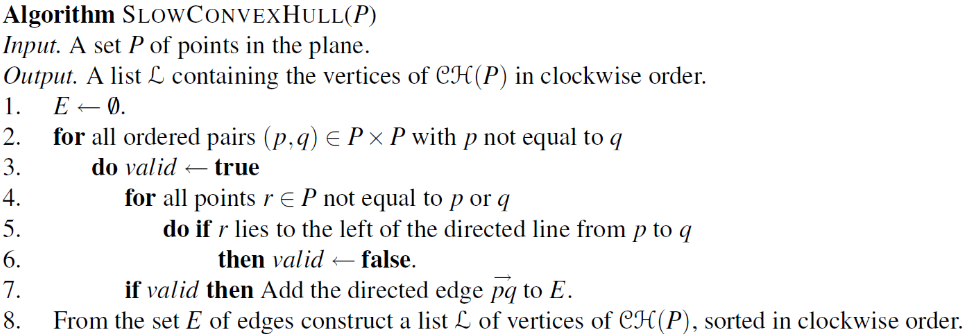
\includegraphics[width=0.9\linewidth]{afbeeldingen/slowconvexhull}
		\label{fig:slowconvexhull}
	\end{figure}
	
	De eerste lus zal $n^2$ keer lopen, gezien het voor elk paar hetgeen in de lus zal uitvoeren. In de lus zelf zal er nog eens over de punten gelopen worden om te kijken of deze allemaal rechts liggen van het gegeven punt, wat nog een $n$ keer zal lopen. De tijdscomplexiteit van dit algoritme is dus $O(n^3)$. 
	
	Naast het feit dat het algoritme helemaal niet efficiënt is, zijn er ook wat problemen in verband met de nauwkeurigheid van het berekenen of zo een punt links of rechts ligt van een ander punt. Het kan zijn dat hierdoor punten fout worden bepaald terwijl ze wel links liggen van een edge. Een ander probleem is wanneer er meerdere punten op een lijn liggen, dit is dan een speciaal geval maar hier zou extra rekening mee gehouden moeten worden, het algoritme zal hier niet automatisch mee omgaan. Dit algoritme is dus duidelijk niet al te efficiënt en er zijn een paar gevallen waarbij het zelfs foute beslissingen kan maken. 
	
	
	\subsection{Incrementeel algoritme 	(Andrew's algorithm)}
	Dit algoritme zal de verzameling punten verdelen in een bovenhelft en in een onderhelft. Deze helften zullen dan in $O(n\log(n))$ volgens de x-as gesorteerd worden. Er zal dan volgens deze sortering gelopen worden om te kijken wanneer er tussen drie punten een 'rechterhoek' of een 'linkerhoek' wordt gemaakt. Als dit onduidelijk is, is hieronder een afbeelding met een voorbeeld waarom die hoeken uitmaken. 
	
	\begin{figure}[h]
		\centering
		\subfigure{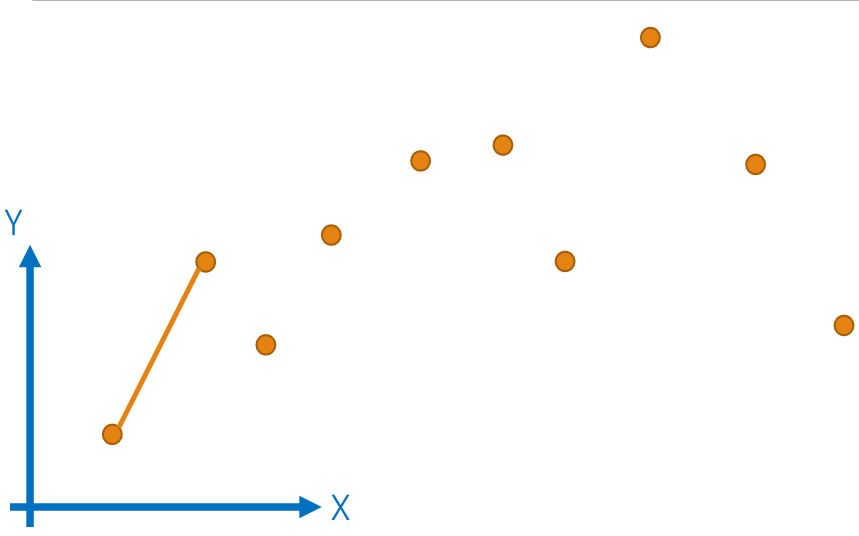
\includegraphics[width=0.24\textwidth]{afbeeldingen/first-convex}} 
		\subfigure{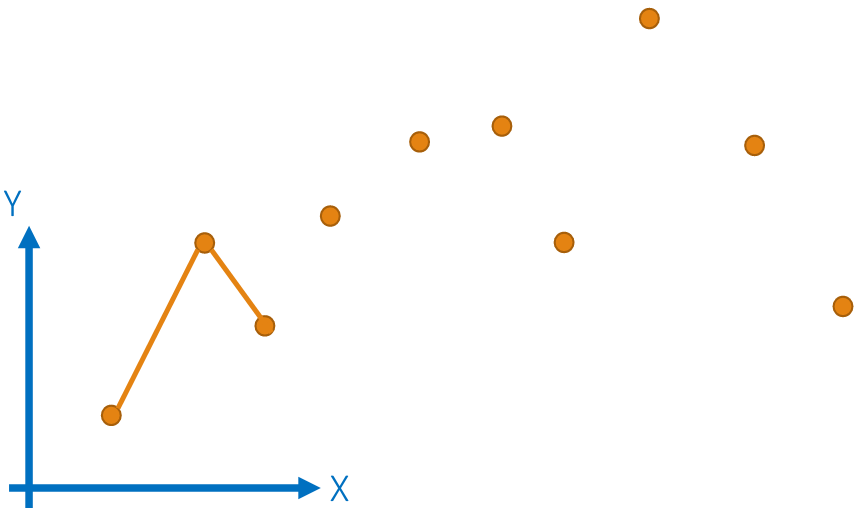
\includegraphics[width=0.24\textwidth]{afbeeldingen/second-convex}} 
		\subfigure{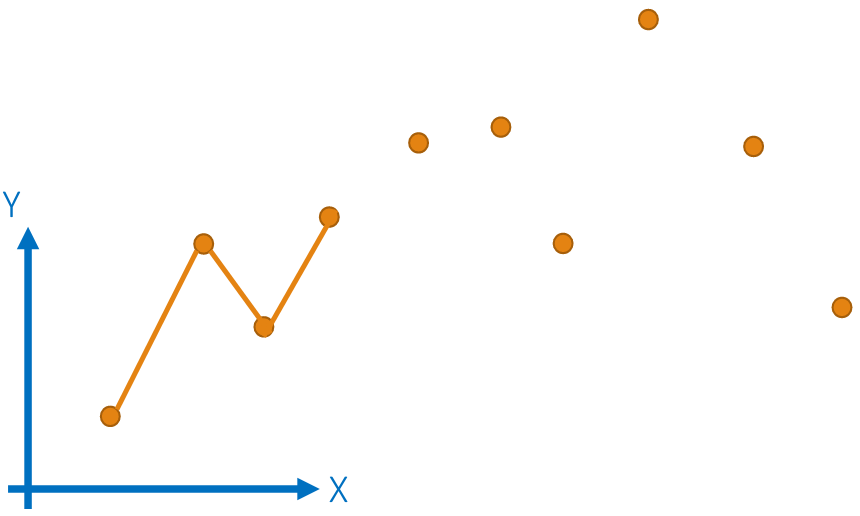
\includegraphics[width=0.24\textwidth]{afbeeldingen/third-convex}}
		\subfigure{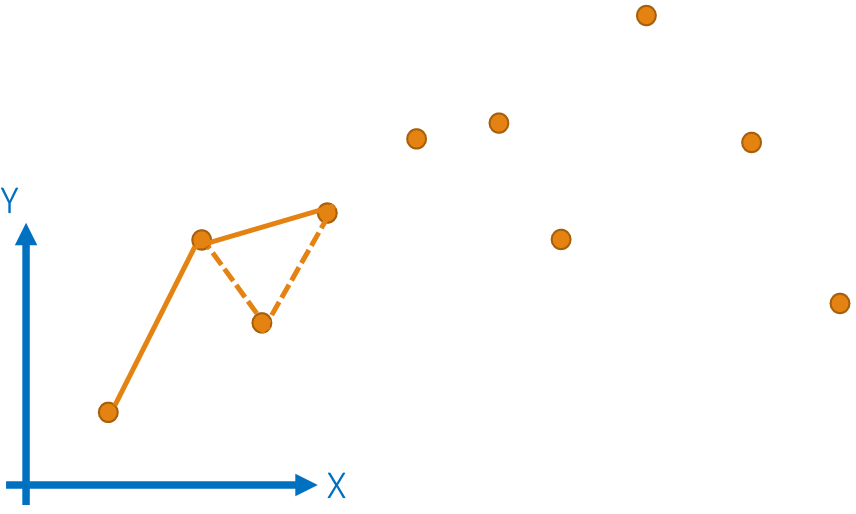
\includegraphics[width=0.24\textwidth]{afbeeldingen/fourth-convex}}
		\label{fig:incremental-example}
	\end{figure}
	Bij afbeelding c maken die punten duidelijk een linkerdraai, wat niet zou mogen voor een convex hull, dus zullen de twee edges verwijderd worden en vervangen worden door de nieuwe. Dit zal voor heel het puntenwolk verdergaan voor de bovenste helft. Voor duidelijkheid is hieronder nog de pseudocode
	\begin{figure}[h]
		\centering
		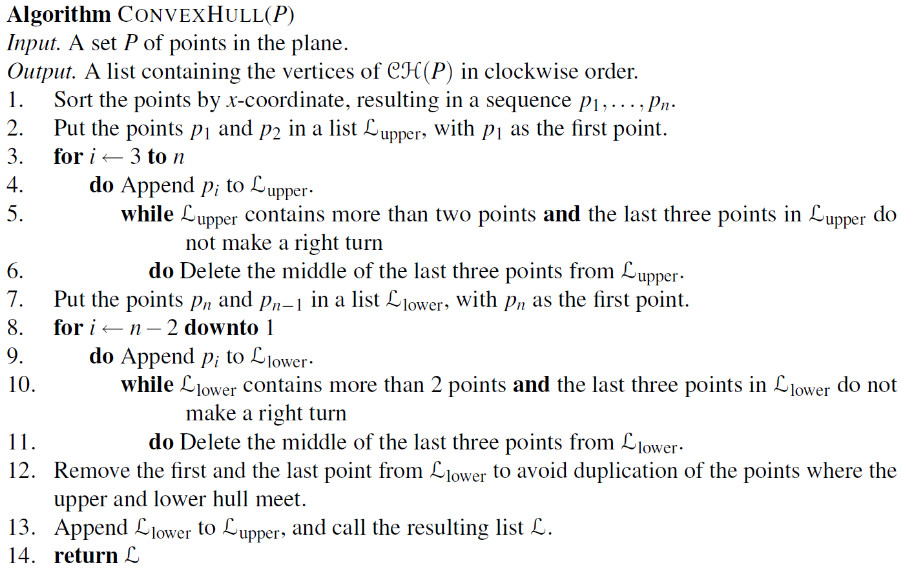
\includegraphics[width=0.9\linewidth]{afbeeldingen/convex-hull}
		\label{fig:convex-hull}
	\end{figure}

	De correctheid van het algoritme wordt bewezen d.m.v inductie: 
	\begin{itemize}
		\item Juiste bovengrens wordt berekend ${p_1, p_2}$
		\item Veronderstel dat we de juiste bovengrens berekend hebben voor ${p_1, p_2, ..., p_{i-1}}$
		\begin{itemize}
			\item $p_i$ toevoegen aan bovengrens - nieuwe bovengrens ligt boven de oude bovengrens
			\item Liggen alle punten ${p_1, p_2, ..., p_i}$ die niet behoren tot de bovengrens, beneden die bovengrens?
			\item Omwille van inductie tot $p_{i-1}$, kan enige mogelijkheid zijn dat een punt tussen $p_{i-1}$ en $p_i$ boven de bovengrens ligt, maar dit is onmogelijk, vermits we punten in gesorteerde volgorde behandelen. 
		\end{itemize}
	\end{itemize}
	Voor de tijdscomplexiteit weten we dat het sorteren van de punten $O(n\log(n))$ zal zijn terwijl voor de rest van het algoritme, we hoogstens één keer over elk punt zullen lopen, wat een tijdscomplexiteit geeft van $O(n)$. De totale tijdscomplexiteit van dit algoritme is dus \(O(n) + O(n\log(n)) = O(n\log(n))\).
	
	Ook voor dit algoritme zijn er speciale gevallen: wat als punten collineair zijn, wat met punten die hetzelfde x-coordinaat hebben en wat als er afrondingsfouten zijn in de hoeken. Dit kan allemaal opgelost worden met extra statements, maar dat geeft een lelijker algoritme. 
	
	
	\subsection{Graham's scan}
	Graham's scan zal niets aan het maken van de convex hull veranderen, maar zal het sorteren aanpassen. De punten zullen gesorteerd worden volgens poolhoek rond laagste meest linkse punt. Na het sorteren zullen de punten volgens de hoek overlopen worden om dan het verdere incrementeel algoritme toe te passen. De eerste van twee afbeeldingen bij Jarvis' march is een goede representatie van hoe de punten gesorteerd worden. 
	
	De tijdscomplexiteit is als volgt te bepalen. Het bepalen van het laagste punt is $O(n)$, het sorteren van de punten volgens punten zal $O(n\log(n))$ vragen en het overlopen zal zoals het vorige algoritme $O(n)$ vragen. De totale tijdscomplexiteit is dus $O(n\log(n))$. 
	
	
	\subsection{Jarvis's March}
	Jarvis' march zal beginnen zoals Graham's scan, beginnen met het uiterst links onderste punt en dan op poolhoeken sorteren, en zal die voor elk punt opnieuw doen. Dit wordt verduidelijkt door de onderstaande afbeeldingen; 
	
	\begin{figure}[h]
		\centering
		\subfigure{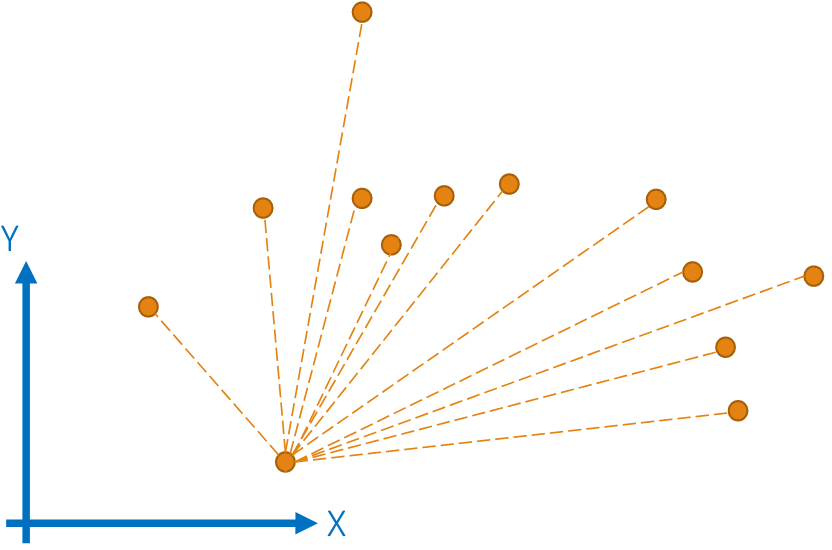
\includegraphics[width=0.45\textwidth]{afbeeldingen/first-jarvis}} 
		\subfigure{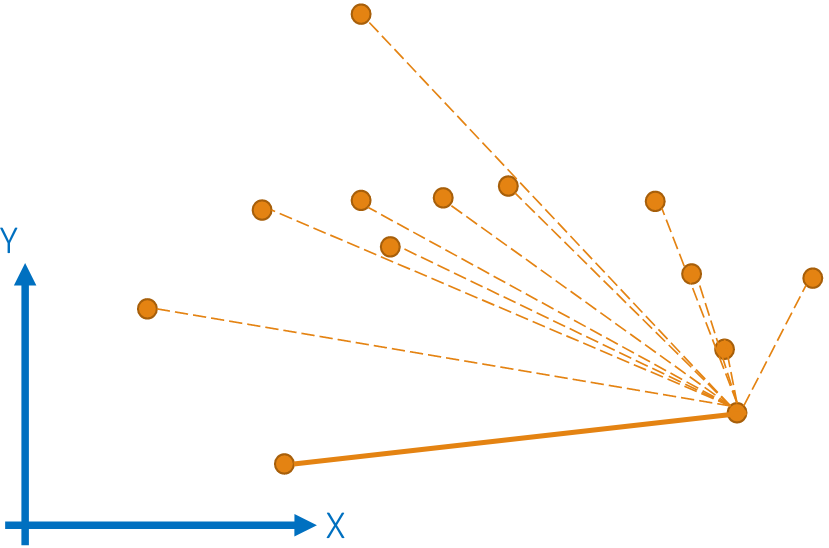
\includegraphics[width=0.45\textwidth]{afbeeldingen/second-jarvis}} 
		\label{fig:jarvis' example}
	\end{figure}

	Voor elk hoekpunt zal gekeken worden naar alle andere punten in de ruimte, hier voelen we aan dat in onze complexiteitsanalyse, we rekening zullen moeten houden met het aantal hoekpunten. Dit is het eerste algoritme waarbij we rekening houden met de output, wat resulteert in een \textit{output-afhankelijke tijdscomplexiteit}. Het aantal hoekpunten en dus het aantal elementen in de output zal in de tijdscomplexiteit $h$ zijn. Gezien we voor elk hoekpunt ongeveer alle andere punten moet overlopen, is de tijdscomplexiteit $O(n\cdot h)$.
	
	Dit algoritme zal dus bijna lineaire tijd hebben bij heel weinig hoekpunten, wat veel beter is dan graham's scan. Anderzijds kan het bijna een kwadratische tijdscomplexiteit worden als het aantal hoekpunten even groot wordt als het algemeen aantal punten. 
	
	Jarvis' march zal bij een klein aantal hoekpunten het logisch algoritme zijn terwijl graham's scan beter is voor een groter aantal. 
	
	%TODO navragen!
	

	\subsection{Verdeel-en-heers}
	Dit is een strategie die we al hebben zien terugkeren bij sorteeralgoritmes. We splitsen het probleem op, we lossen de kleinere problemen op en dan combineren we de oplossingen. De recursie stopt als de verzameling triviaal klein wordt. De tijdscomplexiteit van zo'n algoritmes is vaak $O(n\log(n))$. 
	
	Een manier is om de puntenwolk telkens willekeurig te verdelen en dan de twee convex omhullenden telkens te mergen op de meest extreme punten. Dit lijkt al heel goed, maar willekeurig kan ook heel slechte algoritmes brengen, dus is dit niet altijd het meest ideale. 
	
	Een tweede manier is om de puntenwolk telkens perfect in twee te verdelen volgens de x-coördinaten. De merge-operatie is dan telkens een bovenraaklijn en een onderraaklijn zoeken om deze te verbinden en nog steeds een convex omuhllende te verkrijgen. Deze onder- en bovenbrug is niet altijd het onderste en/of bovenste punt van een puntenwolk, hier bestaat dus een algoritme voor: 
	
	\begin{figure}[h]
		\centering
		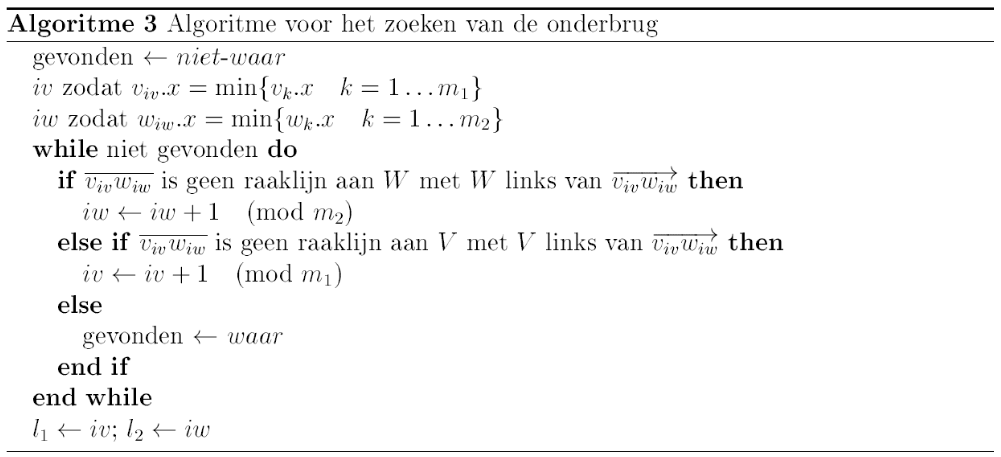
\includegraphics[width=0.9\linewidth]{afbeeldingen/verdeel-en-heers-convex}
		\label{fig:verdeel-en-heers-convex}
	\end{figure}
	%TODO verdere uitleg zoeken want hier zou mondelinge uitleg best ook bijkomen
	
	%TODO Typische examenvragen nog op te lossen
	\subsection{Typische examenvragen}
	\begin{itemize}
		\item \textbf{Leg het Graham Scan algoritme uit voor de berekening van een convex omhullende veelhoek ven een set punten:}\\
		\item \textbf{Hoe zou je Graham's Scan en Jarvis' March met elkaar vergelijken? Wat zijn sterke en zwakke punten van beide algoritmen?:}\\
		\item \textbf{Stel dat je een verzameling punten hebt, waarvan een deel punten  colineair zijn (ttz op dezelfde lijn liggen). Welke problemen zou je kunnen ontmoeten bij het Graham's Scan algoritme? Bij Jarvis' March?:}\\
		\item \textbf{Stel dat je de convex omhullende wil berekenen van een set van n lijnsegmenten. Hoe zou je dit aanpakken?:}\\
		\item \textbf{Zou je het verdeel-en-heers algoritme ook kunnen toepassen als je de verzameling punten in 4 verdeelt - bijvoorbeeld zowel via de x-mediaan als de y-mediaan? Op welke manier kan je dan 4 convex omhullende veelhoeken combineren tot 1 veelhoek?:}\\
		\item \textbf{Bij het verdeel-en-heers algoritme kan je zowel een verdeling van de x-mediaan als volgens de y-mediaan toepassen. Op alle recursieve niveau's zou je telkens een andere beslissing kunnen nemen (verdelen volgens x of y). Van welke factoren zou deze keuze kunnen afhangen?:}\\
		\item \textbf{In welke mate is algoritme *vul hier een convex omhullende algoritme in * bestand tegen kleine rekenfouten? Levert het algoritme telkens een gesloten veelhoek? Soms zelfs geen veelhoek? Een concave veelhoek? Wat zijn mogelijke oorzaken van dergelijke fouten?:}\\
	\end{itemize}


	\section{Intersecties van lijnstukken}
	In dit hoofdstuk worden algoritmes besproken om snijpunten tussen lijnstukken te vinden. 
	\subsection{Brute Force algoritme}
	Het brute force algoritme zal domweg, zoals wel verwacht, elk lijnstuk met elk ander evalueren op een snijpunt. De pseudocode ervoor is hier te vinden:
	\begin{figure}[h]
		\centering
		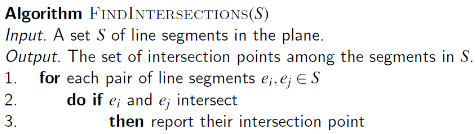
\includegraphics[width=0.8\linewidth]{afbeeldingen/find-Intersections}
		\label{fig:find-intersections}
	\end{figure}
	Het is duidelijk dat de tijdscomplexiteit van dit algoritme dus altijd $O(n^2)$ zal zijn en dat dit een \textit{input-afhankelijke tijdscomplexiteit} heeft. Wanneer elk lijnstuk met elkaar snijdt kan dit geen kwaad, maar als geen enkel lijnstuk met een ander snijdt, zal je hier heel veel tijd mee verliezen. 
	
	
	\subsection{Doorlooplijn algoritme}
	%TODO stel u voor, ge weet ondertussen nog niet wat een doorlooplijn is
	Een doorlooplijn is een denkbeeldige lijn die door de dataset loopt en bijhoudt welke lijnsegmenten actief zijn en dus potentieel elkaar kunnen snijden. Als twee lijnsegmenten op die lijn zitten kan het zijn dat ze elkaar snijden, als ze niet op een moment gelijktijdig op de lijn zitten, is er geen kans dat ze elkaar snijden en moeten ze dus niet geëvalueerd worden op snijpunten. Als eerste zullen de punten dus gesorteerd moeten worden op de y-as volgens de begin- en eindpunten van de lijnsegmenten. Deze zouden dan terechtkomen in een event queue om deze af te lopen en bij elk punt een actie te ondernemen. Bij een startpunt worden alle actieve lijnsegmenten geëvalueerd met het nieuwe toegevoegde lijnsegmenten om snijpunten te zoeken. Zo wordt een deel van de lijnsegmenten gefilterd en is het geen bruteforce. De datastructuur voor de doorlooplijn zou in dit geval gewoon een set kunnen zijn aangezien deze niet gesorteerd hoeven te zijn. 
	
	De worst case van dit algoritme is wanneer er allemaal lijnstukken parallel verticaal naast elkaar liggen. Dan wordt elk lijnstuk met elkaar vergeleken ondanks dat we een doorlooplijn gebruiken en is het even onefficiënt als een brute force algoritme. 
		
	\subsection{Doorlooplijn++}
	In de verbeterde doorlooplijn zullen we niet naar alle actieve lijnstukken kijken op de lijn, maar enkel naar de buren van het toegevoegde lijnstuk. Nu zal er dus wel een datastructuur nodig zijn om deze sortering bij te houden, dit zal het beste gaan met een gebalanceerde zoekboom. Er zijn verschillende soorten 'events' in dit algoritme, je kan van elk een voorbeeld zien in de onderstaande afbeelding.  
	
	\begin{figure}[h]
		\centering
		\subfigure{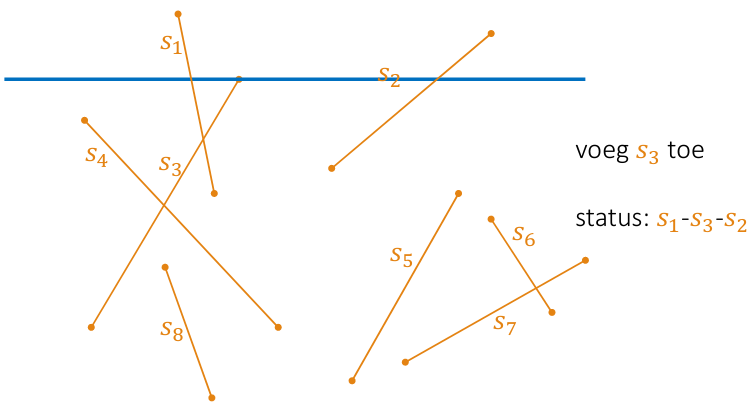
\includegraphics[width=0.24\textwidth]{afbeeldingen/first-doorlooplijn}} 
		\subfigure{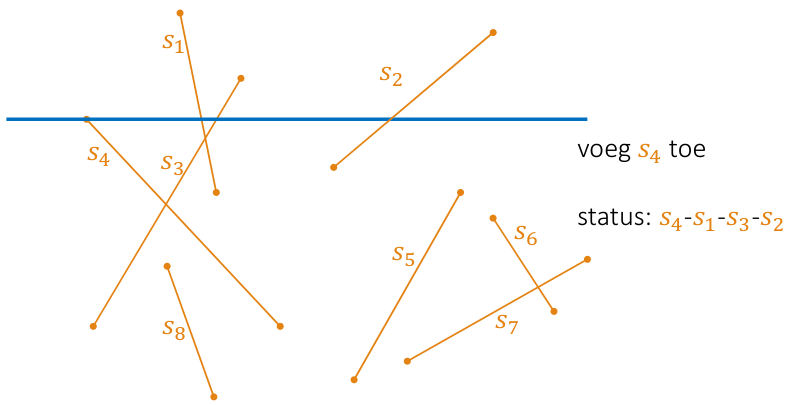
\includegraphics[width=0.24\textwidth]{afbeeldingen/second-doorlooplijn}} 
		\subfigure{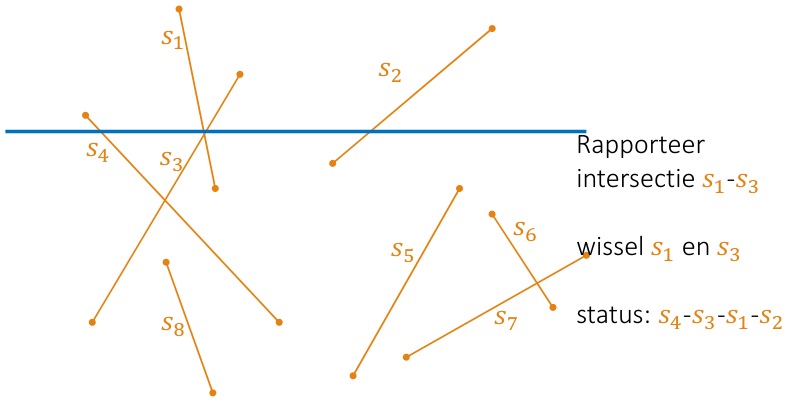
\includegraphics[width=0.24\textwidth]{afbeeldingen/third-doorlooplijn}}
		\subfigure{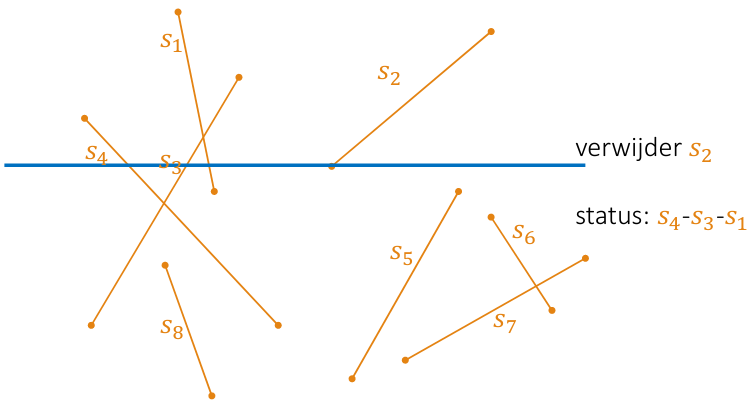
\includegraphics[width=0.24\textwidth]{afbeeldingen/fourth-doorlooplijn}}
		\label{fig:sweepline-example}
	\end{figure}

	De event queue zal in dit geval ook een gebalanceerde zoekboom zijn, het is geen priority queue aangezien er niets is dat een 'prioriteit' heeft.
	\begin{description}
		\item[Start event:] Een start event is wanneer een nieuw lijnstuk actief wordt op de doorlooplijn, in dat geval zal het nieuwe lijnstuk vergeleken worden met zijn buren op snijpunten. Als er snijpunten worden gevonden, worden deze toegevoegd aan de event queue. 
		\item[Intersection event:] Bij een snijpunt zal het algoritme de volgorde van de lijnstukken op de status queue verwisselen en deze lijnstukken zullen dan met hun nieuwe buren vergeleken worden voor nieuwe snijpunten. 
		\item[End event:] Het einde van een lijnstuk betekent dat dit lijnstuk van de status queue gehaald moet worden en dat er moet gekeken worden of de nieuwe buren elkaar snijden. 
	\end{description}

	De pseudocode is hieronder te vinden: 
	
	\begin{figure}[h]
		\centering
		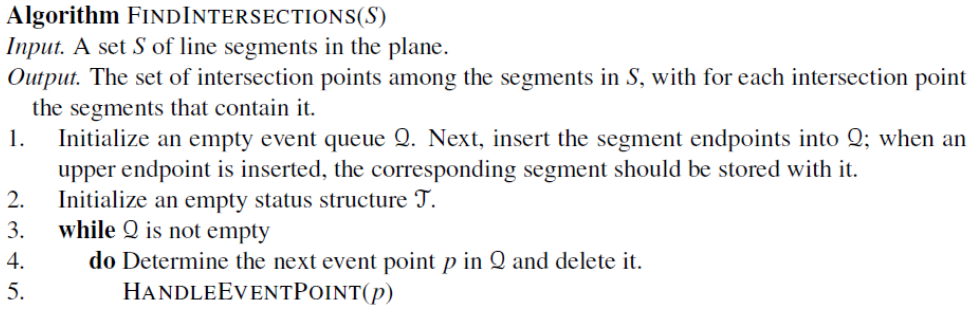
\includegraphics[width=0.9\linewidth]{afbeeldingen/find-intersections++}
		\label{fig:find-intersections++}
	\end{figure}
	
	De correctheid van dit algoritme wordt als volgt bewezen: Indien twee lijnsegmenten elkaar snijden, moet er ergens een event zijn boven het intersectiepunt, waar beide lijnsegmenten elkaars buren worden.\\
	Indien de doorlooplijn zich net boven een intersectiepunt p bevindt, zijn $s_i$ en $s_j$ aangrenzend (en worden dus getest op intersectie).\\
	Initieel is de status leeg, er moet dus ergens een event zijn dat $s_i$ en $s_j$ aangrenzend maakt.
	
	Elk event is begrensd door een tijdscomplexiteit van $O(\log(n))$. De lus zal 2n + k keer uitgevoerd worden, met $n$ het aantal cirkels en $k$ het aantal snijpunten. De lus zal dus  $O(n + k)$ overlopen worden, wat een totaal geeft van $O((n+k)\log(n))$. Qua geheugen zal de status vast zijn door het maximaal aantal elementen dat er op de lijn tevoorschijn kan komen, wat dus $O(n)$ is. De event queue zal begrensd zijn door $2n + k$ events, wat in het ergste geval kan uitkomen op $O(n^2)$. 
	
	Een speciaal geval kan twee punten zijn die dezelfde y-waarde hebben, dan kan de event queue het niet juist sorteren. Dit kan opgelost worden door de doorlooplijn zogezegd wat schijner te laten lopen. Een ander probleem is het samenvallen van events (het einde van een lijnstuk is gelijk aan het begin van een ander lijnstuk.) Hier moeten dan tijdens het implementeren bepaalde keuzes gemaakt worden, maar dit kan ook opgelost worden. %TODO moet hier nog iets bij? 


	\subsection{Doubly-connected edge list}
	Een DCEL is een manier om een oppervlak met lijnen in een datastructuur te steken en zo gemakkelijk over de datastructuur kunnen verplaatsen. Eerst volgen wat termen die belangrijk zijn om te kunnen praten over deze DCEL. 
	
	\begin{figure}[H]
		\centering
		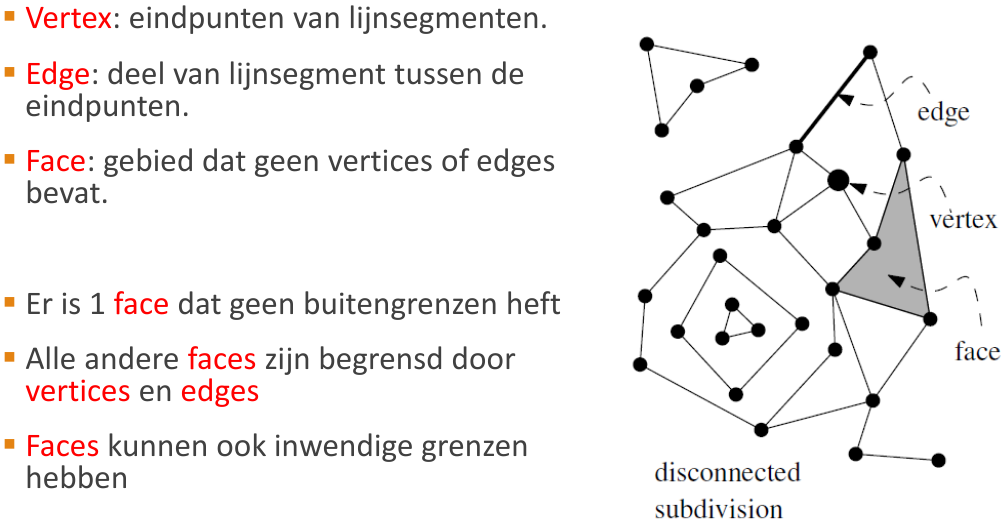
\includegraphics[width=0.8\linewidth]{afbeeldingen/DCEL-termen}
		\label{fig:dcel-termen}
	\end{figure}

	Het centrale idee is dat elke edge uit bovenstaande afbeelding kan gemaakt worden uit 2 'half-edges'. Deze half edges hebben elk een oorsprong-vertex, een twin (de andere half edge), een incidentface (face aan de linkerkant van de half-edge), een next en een prev. Elke vertex bestaat uit coördinaten en een incidentEdge (de edge startende in de vertex). 
	
	Met deze datastructuur kunnen we gemakkelijker de overlay van twee vlakverdelingen bepalen. Dit is eigenlijk aanvankelijk het construeren van een DCEL uit twee DCEL's, wat door een doorloopalgoritme zal gebeuren. Ook hier werken we met events: 
	\begin{itemize}
		\item Een vertex van S1
		\item Een vertex van S2
		\item Een intersectiepunt van een edge van S1 met een edge van S2. 
		\begin{figure}[H]
			\centering
			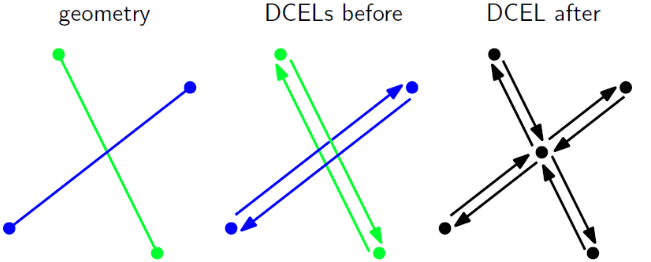
\includegraphics[width=0.7\linewidth]{afbeeldingen/intersection-DCEL}
			\label{fig:intersection-dcel}
		\end{figure}
		\item De edge van S1 snijdt met een vertex van S2 (of omgekeerd)
		\begin{figure}[H]
			\centering
			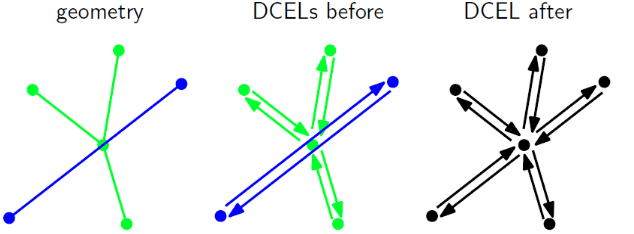
\includegraphics[width=0.7\linewidth]{afbeeldingen/DCEL-vertex&edge}
			\label{fig:dcel-vertexedge}
		\end{figure}
		\item Samenvallende vertices van S1 en S2
		\begin{figure}[H]
			\centering
			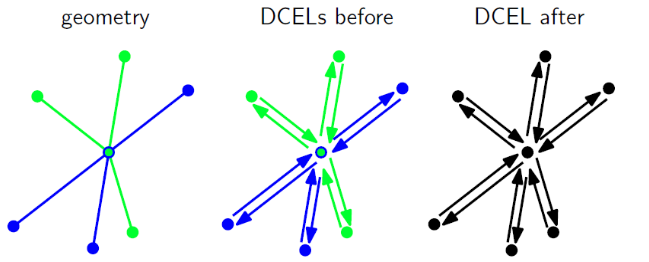
\includegraphics[width=0.7\linewidth]{afbeeldingen/DCEL-vertices}
			\label{fig:dcel-vertices}
		\end{figure}
	\end{itemize}

	Om de faces te bepalen, zal de nieuwe DCEL overlopen moeten worden om alle loops te detecteren en de inwendige en uitwendige grenzen te bepalen. Een face moet dan geconstrueerd worden voor elke uitwendige grens (+ het buitengebied). Van de inwendige grenzen kunnen we het meest links punt bepalen (van de vorm) en zodra een andere edge is gevonden, wordt deze vorm overlopen. Dit is dan de vorm waarbinnen de aanvankelijke vorm ligt. Dan kan een structuur zoals hieronder gemaakt worden. Deze indelingen zijn gemakkelijk om booleaanse opdrachten te gebruiken op veelhoeken.
	
	\begin{figure}[H]
		\centering
		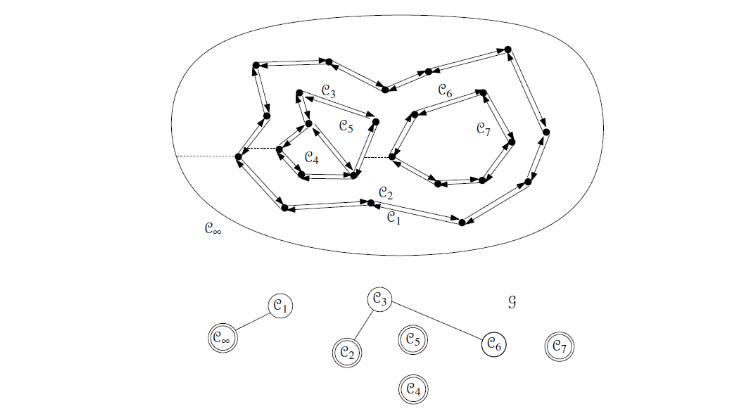
\includegraphics[width=0.7\linewidth]{afbeeldingen/DCEL-faces}
		\label{fig:dcel-faces}
	\end{figure}
	
	Voor de tijdscomplexiteit is de volgende afbeelding het bewijs (cuz ja, ik ben effe lui):
	
	\begin{figure}[H]
		\centering
		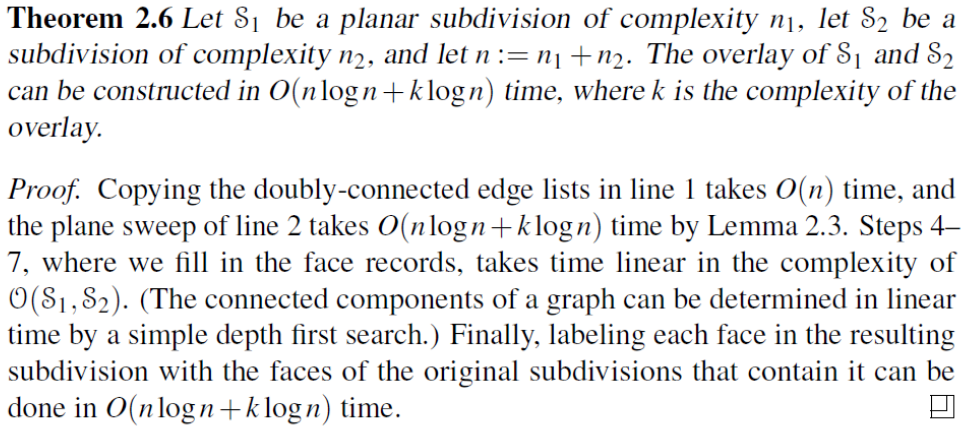
\includegraphics[width=0.7\linewidth]{afbeeldingen/DCEL-bewijs}
		\label{fig:dcel-bewijs}
	\end{figure}
	
	
	\subsection{Typische examenvragen}
	\begin{itemize}
		\item \textbf{Wat is de algemene idee van sweep-line algoritmen?:}\\
		\item \textbf{Beschrijf het algoritme om alle intersectiepunten in een verzameling lijnstukken te vinden. Bespreek ook de tijdscomplexiteit:}\\
		\item \textbf{Bespreek de Double-Connected-Edge-List als datatstructuur. Wat zijn voor- en nadelen van deze datastructuur?:}\\
		\item \textbf{Bespreek welke operaties er precies moeten gebeuren bij de afhandeling van <event van type X> bij het berekenen van de overlay van 2 vlakindelingen:}\\
	\end{itemize}
	
	
	\section{Triangulaties van veelhoeken}
	Dit deel begint met een klein voorbeeld als context. Stel dat je in een museum werkt en moet besluiten waar de bewakers 's nachts zullen staan. Je wilt natuurlijk zo min mogelijk (stilstaande) bewakers voor de ruimte die je moet bewaken. Dit wordt het \textit{Museumprobleem} genoemd. Bij deze probleemstelling komen dan ook de vraag: Wat is het minimaal aantal bewakers dat nodig is voor een n-hoek? Hier wordt dan ook een max over min forumlering gebruikt: Wat is het grootste aantal bewakers dat een veelhoek minimum nodig heeft? Je kan een 12-hoek bijvoorbeeld opdelen met 1 bewaker en met 4 bewakers, het maximum van de minima is hier 4 en dat is wat we dan zoeken. Dit getal schrijven we als $G(n)$ met n het aantal hoeken. Wat vanzelfsprekend is, is dat $G(n) \geq 1$ en dat $G(n) \leq n$ maar dit is te algemeen, we moeten specifieker gaan zoeken. Na een aantal voorbeelden is het duidelijk dat dit getal gelijk is aan $\lfloor n/3\rfloor$. Dit is dus het aantal bewakers dat voor een veelhoek met n hoeken altijd genoeg zal zijn om heel de ruimte te bewaken. 
	
	\subsection{Triangulaties}
	Een triangulatie is het toevoegen van zo veel mogelijk niet snijdende diagonalen in de veelhoek. Een diagonaal is een lijnstuk tussen twee hoekpunten die strikt zichtbaar zijn tegenover elkaar. Zoals je wel al merkt is zo een triangulatie niet uniek, er bestaan er heel veel en er is niet één juiste. Wat we met zekerheid kunnen zeggen is dat elke veelhoek kan getrianguleer worden om uit te komen op $n-2$ driehoeken. We bewijzen die door middel van inductie: 
	- $n-3$ : triviaal (1 driehoek wordt getrianguleerd in 1 driehoek).\\
	- $n > 3$ : 
	\begin{itemize}
		\item We construeren een diagonaal in $P$:
		\begin{itemize}
			\item $v$ is meest linkse vertex van $P$, met buren $u$ en $w$
			\item Geval 1: Indien $\overline{uw}$ binnen $P$ ligt $\rightarrow$ $\overline{uw}$ is een diagonaal
			\item Geval 2: er liggen vertices van $P$ binnen de driehoek $\vartriangle uw$:
			
			neem $v'$ als verst verwijderde van de lijn $\overline{uw}$. $\overline{vv'}$ kan $P$ niet snijden $\rightarrow$ $\overline{vv'}$ is een diagonaal. 
		\end{itemize}
		\item De diagonaal verdeelt $P$ in $P_1$ en $P_2$, met $m_1$ en $m_2$ vertices
		\item (veronderstel dat de stelling geldt voor $m<n)$
		\begin{itemize}
			\item $P_1$: $m_1$ vertices, triangulatie in $m_1$-2 driehoeken. 
			\item $P_2$: $m_2$ vertices, triangulatie in $m_2$-2 driehoeken. 
			\item $m_1 - m_2 = n+2$
		\end{itemize}
		\item $\rightarrow$ Triangulatie van $P$ telt $(m_1 -2) + (m_2 - 2) = n-2$ driehoeken. 
	\end{itemize}
	In het museumprobleem kunnen we gebruik maken van deze triangulatie: 
	\begin{figure}[H]
		\centering
		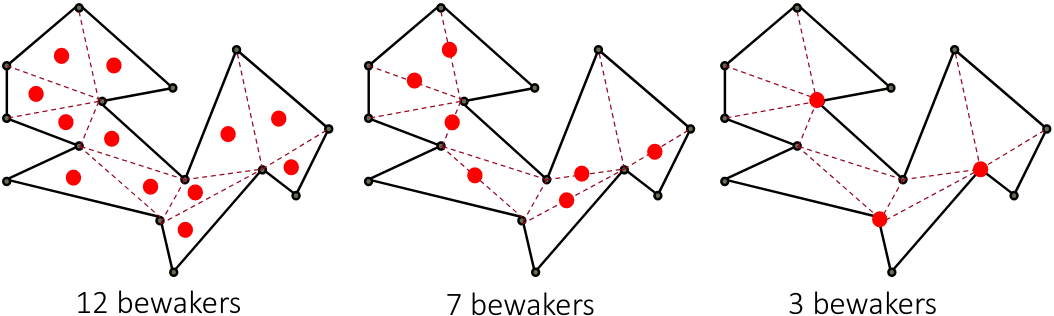
\includegraphics[width=0.9\linewidth]{afbeeldingen/triangulatie-bewakers}
		\label{fig:triangulatie-bewakers}
	\end{figure}
	Het is duidelijk dat de laatste figuur zorgt voor een optimale oplossing: zo weinig mogelijk bewakers die nog steeds de volledige ruimte in het oog kunnen houden. Het vinden van deze perfecte plekken kan aan de hand van een 'kleuring'. 
	
	
	\subsection{kleuring}
	Een kleuring is het toekennen van kleuren aan vertices zodat verbonden vertices een verschillende kleur hebben. Voor onze situatie gebruiken we een 3-kleuring, elke vertex mag dus een van die drie kleuren hebben. Zo en kleurring kan gemakkelijk gevonden worden door telkens een driehoek te halen uit de triangulatie, elke keer als die driehoek terug toegevoegd moet worden zal de nieuwe hoek die nog geen kleurring heeft, eenduidig bepaald een van de drie kleuren bevatten. Na het kleuren van de vertices kan je dan besluiten een van de kleuren te kiezen om dan de bewakers daar te positioneren. Het is ergens wel logisch dat er van sommige kleuren meer zijn dan anderen, net zoals hiernoder te zien is. 
	\begin{figure}[h]
		\centering
		\subfigure{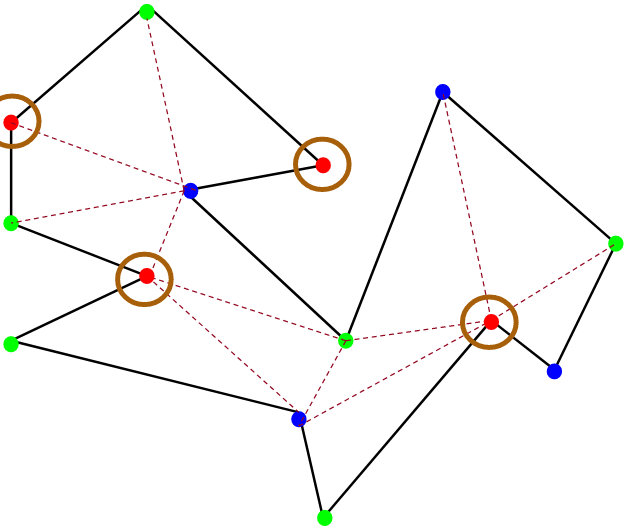
\includegraphics[width=0.32\textwidth]{afbeeldingen/triangulatie-rood}} 
		\subfigure{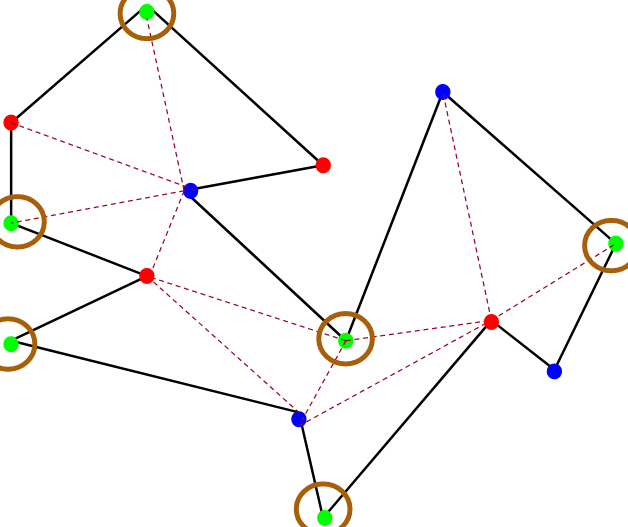
\includegraphics[width=0.32\textwidth]{afbeeldingen/triangulatie-groen}} 
		\subfigure{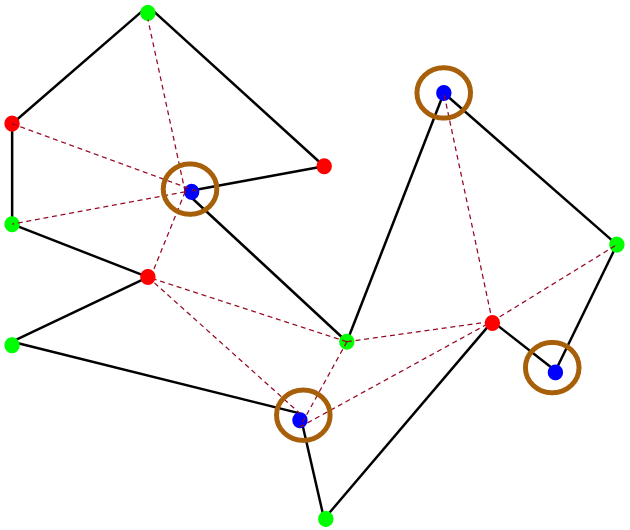
\includegraphics[width=0.32\textwidth]{afbeeldingen/triangulatie-blauw}}
		\label{fig:trianuglation-colours}
	\end{figure}
	Het is hier duidelijk dat rood en blauw elk een goeie verdeling hebben, maar ook niet allebei optimaal. Bij beiden zou er nog een bewaker kunnen wegvallen en zou heel het oppervlak nog steeds bewaakt zijn. Gezien dit een 3-kleuring is, wordt elke kleur maximaal $n/3$ keer gebruikt en vermits $n$ geheel is: $\lfloor n/3 \rfloor$. Een goede voorstelling hiervan is ook Chvátal's kam. 
	\begin{figure}[H]
		\centering
		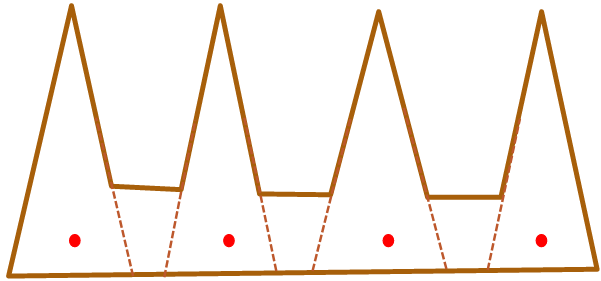
\includegraphics[width=0.6\linewidth]{afbeeldingen/triangulatie-kam}
		\label{fig:triangulatie-kam}
	\end{figure}

	Het is duidelijk dat dit het ergste geval is. We weten nu de theorie achter deze triangulaties, maar we moeten nog ontdekken hoe we deze moeten opstellen. 
	
	
	\subsection{Hoe te trianguleren}
	Het trianguleren begint best door elke keer een oor af te snijden en zo verder te zoeken naar een triangulatie binnen de nieuwe veelhoek met $n-1$ vertices. De tijdscomplexiteit van die algoritme zou dan $O(n^2)$ zijn. Voor convexe veelhoeken wordt die zelfs $O(n)$. 
	
	Om een veelhoek te trianguleren beginnen we eerst met het definiëren van een 'y-monotone' veelhoek. Een veelhoek is y-monotoon als een horizontale lijn de veelhoek over slechts één interval snijdt. De veelhoek wordt opgesplitst in y-monotone veelhoeken en van elk van deze veelhoeken wordt dan de triangulatie gezocht. In een veelhoek kan elke hoek ingedeeld worden als volgt: 
	\begin{figure}[H]
		\centering
		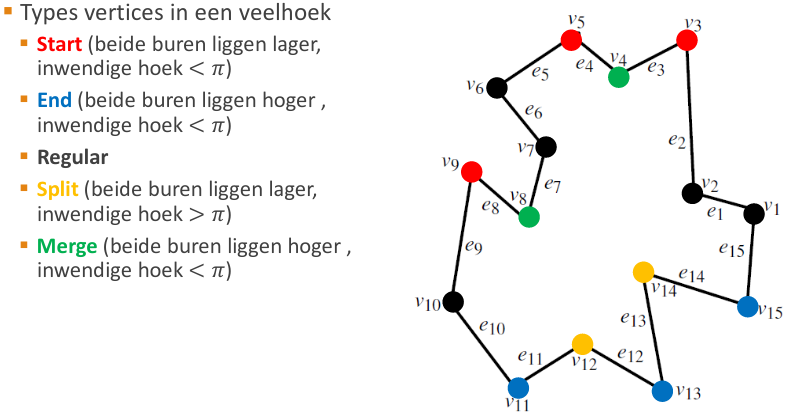
\includegraphics[width=0.7\linewidth]{afbeeldingen/triangulaties-y-monotoon}
		\label{fig:triangulaties-y-monotoon}
	\end{figure}
	Het is relatief duidelijk dat de split en merge knopen het probleem vormen om de veelhoek y-monotoon te maken. Wanneer een veelhoek niet y-monotoon is, is het duidelijk dat het of een split node heeft, of een merge node, deze zullen we moeten wegwerken met een algoritme. Het algoritme zal dan een diagonaal maken bij merge-vertices die naar beneden gaat, en bij split-vertices die naar boven gaat. Dit zal, you guessed it, met een doorlooplijn algoritme gebeuren. Hierbij initialiseren we een helper voor een edge, deze helper is de laatste vertex boven de doorlooplijn, waarbij de horizontale tussen de edge en de vertex volledig binnen de veelhoek ligt. 
	
	Om een merge vertex juist op te lossen, kijk je telkens er een nieuwe helper wordt geïnitialiseerd, of de oude helper een merge vertex is. Als die een merge vertex is, dan zal de oude en de nieuwe helper verbonden worden. Een split vertex zal gelijkaardig opgelost worden, maar dan zal de split een nieuwe helper zijn en wordt deze verbonden met de oude helper. Dit algoritme kan gebeuren in $O(n\log(n))$ met het geheugen in lineaire tijd. 
	
	De triangulatie van de overbleven monotone veelhoeken kan dan gedaan worden met een greedy algoritme. We sorteren de vertices volgens y-coördinaat en zetten de twee eerste vertices op de stack. Daarna wordt er zo veel mogelijk getrianguleerd naar wat er op de stack staat. Dit geldt voor alle geldige diagonalen op de stack. Zodra er een ongeldige diagonaal is, wordt er naar de laatste vertex gekeken en van daar uit nieuwe diagonalen maken. Hier is een goede illustratie van in de slides. 
	
	Dit algoritme werkt in lineaire tijd $\rightarrow$ $O(n)$. Met het algoritme om de veelhoek in te delen in monotone veelhoeken zal de totale complexiteit $O(n\log(n))$ zijn. 
	
	
	\subsection{Typische examenvragen}
	\begin{itemize}
		\item \textbf{Bewijs dat een oplossing voor het “museumprobleem” of “art gallery problem” voor een (eenvoudige) veelhoek met n hoeken een bovengrens heeft gelijk aan  n/3 (naar beneden afgerond) bewakers:}\\
		\item \textbf{Stel dat we een klasse (eenvoudige) veelhoeken hebben, met als eigenschap dat ze d.m.v. niet-snijdende diagonalen in de veelhoek steeds kunnen opgesplitst worden in een verzameling convexe vierhoeken. Welke uitspraken kan je doen i.v.m. het “museumprobleem” of “art gallery problem” voor deze klasse van veelhoeken?:}\\
		\item \textbf{Bewijs dat elke eenvoudige veelhoek met n hoekpunten kan getrianguleerd worden in n-2 driehoeken. Geef duidelijk alle stappen in de redenering:}\\
		\item \textbf{Op welke manier kunnen we een veelhoek splitsen in een aantal monotone veelhoeken?:}\\
		\item \textbf{In het globale algoritme om een veelhoek te trianguleren splitsen we eerst de veelhoek op in y-monotone veelhoeken. Maakt het een verschil voor de finale triangulatie als we zouden splitsen in x-monotone driehoeken?:}\\
	\end{itemize}
	
	
	\section{Lineaire programming \& gerandomiseerde algoritmen}
	De probleemstelling van het eerste deel van dit stuk is: Kan een bepaald ontwerp gemaakt worden met één enkele gietvorm en kan dat object in één vloeiende beweging verwijderd worden. De probeemstelling is gevisualiseerd als volgt: 
	\begin{figure}[H]
		\centering
		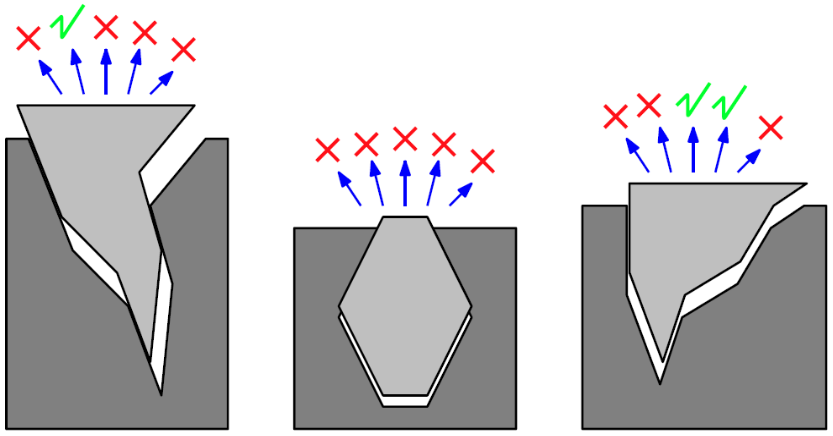
\includegraphics[width=0.6\linewidth]{afbeeldingen/gietvorm-voorbeeld}
		\label{fig:gietvorm-voorbeeld}
	\end{figure}
	
	De richting kan ook voorgesteld worden door pijlen in een bepaalde richting (geprojecteerd op $y=1$). Daar waar de richtingen overlappen, kan je dan naar boven trekken aan de vorm en zal je die in één keer eruit kunnen halen. Op dezefde manier kan die op een vlak geprojecteerd worden voor een 3d vorm. Hier hoort ook een lemma bij (dat ik zelf nog niet volledig snap)
	\begin{figure}[H]
		\centering
		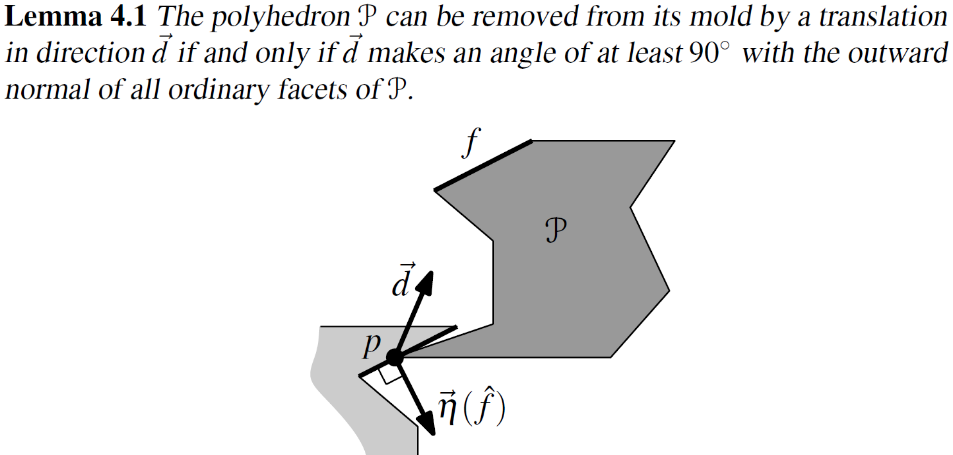
\includegraphics[width=0.7\linewidth]{afbeeldingen/gietvorm-lemm}
		\label{fig:gietvorm-lemma}
	\end{figure}
	
	Geldige richtingen in 3d kunnen voorgesteld worden door $n-1$ hafvlakken, met n het aantal vlakken van de vorm (waarbij -1 staat voor het bovenste vlak). De algemene vraag is dan: bereken de verzameling punten die beantwoorden aan alle constraints. Een interessante observatie is dat elk van die doorsnedes altijd een convexe vorm zal zijn. 
	
	
	\subsection{intersectie van halfvlakken}
	
	\begin{description}
		\item[Brute force]:\\
			Dit algoritme zal recursief berekenen wat de doorsnede is en gebruikt dan DCEL's om deze opnieuw te mergen. De pseudocode zal dit duidelijker maken: 
			\begin{figure}[H]
				\centering
				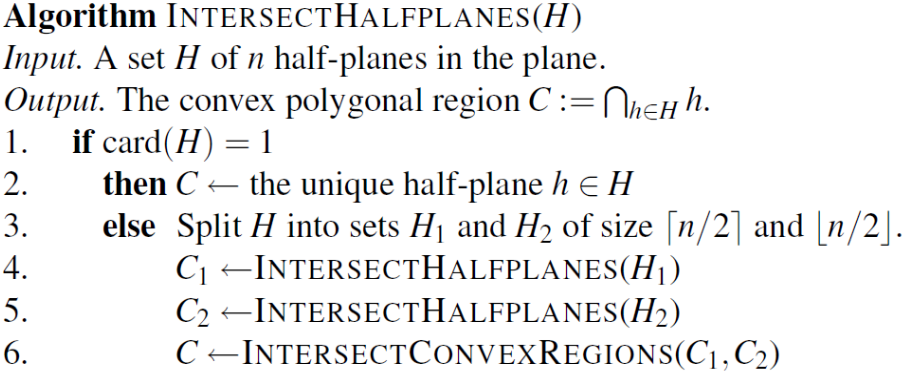
\includegraphics[width=0.8\linewidth]{afbeeldingen/intersectHalfPlanes}
				\label{fig:intersecthalfplanes}
			\end{figure}
			
		\item[Doorlooplijn]:\\
			Hier moet niet echt veel uitleg meer bij, het is gewoon een doorlooplijn die de linker- en rechterkant zal updaten met snijpunten als events.  
		\item[Incrementeel]:\\
			Voor het probleem van de gietvorm, is het genoeg één oplossing te kennen, en niet de volledige doorsneden. Alle halfvlakken kunnen gerepresenteerd worden door een vergelijking die groter moet zijn dan een bepaalde waarde, wat dus een rechte zal geven met een helft die wel mag gelden. We definiëren dan een functie f die afhankelijk is aan deze constraints en als we f maximaliseren, zullen we een bepaalde waarde hebben die deel is van de doorsnede. Het kan ook zijn dat we f blijven maximaliseren, maar dit zal uitkomen op een edge van de doorsneden, of zelfs tot in het oneindige voort zal gaan. 
			
			Dit algoritme is gelijkaardig aan een voor een een halfvlak toevoegen en veronderstellen dat de oplossing uniek is. Er zullen dus ook twee halfvlakken moeten geplaatst worden op de randen om de onbegrensde gevallen ook in rekening te brengen. Als bij het toevoegen van een halfvlak, de vertex nog steeds tot de doorsnede behoort: behouden we die vertex, anders moet er een nieuwe vertex gezocht worden. 
			\begin{figure}[H]
				\centering
				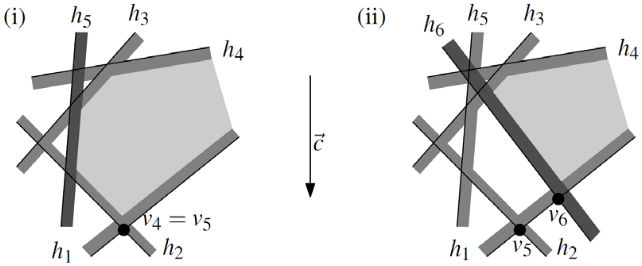
\includegraphics[width=0.7\linewidth]{afbeeldingen/gietvorm-incrementeel}
				\label{fig:gietvorm-incrementeel}
			\end{figure}
			
			De worst case is wanneer de vertex telkens opnieuw geplaatst moet worden, dan wordt de tijdscomplexiteit $O(n^2)$.
		\item[Random incrementeel]:\\
			Dit algoritme zal hetzelfe doen als het vorige, maar deze keer de halfvlakken willekeurig toevoegen. De kans bij een willekeurig halfvlak is $\frac{(i-2)}{i}$ de kans dat de laatste toevoeging een goedkope stap is. De tijdscomplexiteit zou dan $\sum_{i=1}^n O(i)\cdot\frac{2}{i} = O(n)$.
	\end{description}
	
	
	\subsection{kleinst omsluitende cirkel}
	Gegeven een set punten, wat is de kleinst omsluitende cirkel die je daarrond kan trekken. Een logische observatie is dat er een aantal punten op de cirkel zullen moeten liggen, anders is de cirkel niet minimaal. Specifieker zelfs: er zullen telkens minstens 3 punten op die cirkel liggen. Andere eigenschappen zijn: 1) De kleinst omsluitende cirkel is uniek, 2) indien een punt binnen in de cirkels weggehaald wordt, zal de cirkel zelf niet veranderen en 3) In dien een punt buiten de cirkel ligt, komt dat punt op de cirkel te liggen. 
	
	Dit probleem kan ook opgelost worden met een willekeurig incrementeel algoritme. Dit betekent dat er willekeurig telkens een punt zal toegevoegd worden en een voor een. Hierbij is het volgend lemmma belangrijk: 
	\begin{figure}[H]
		\centering
		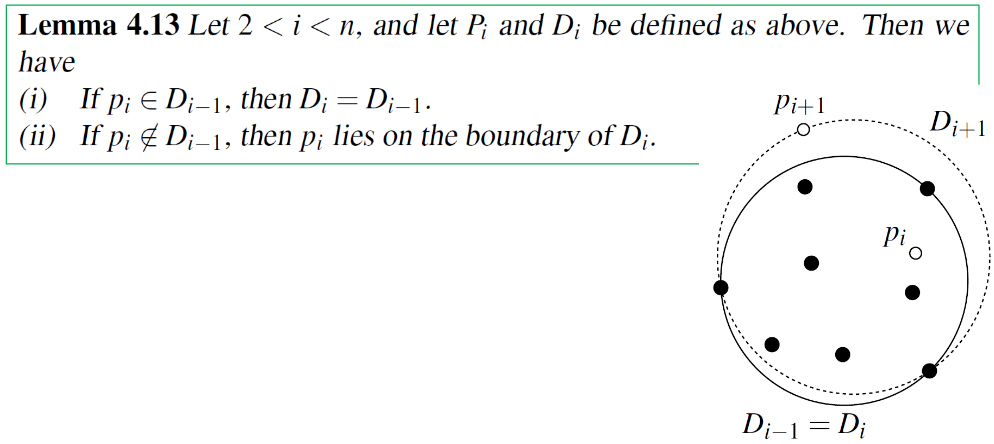
\includegraphics[width=0.8\linewidth]{afbeeldingen/cirkel-lemma}
		\label{fig:cirkel-lemma}
	\end{figure}
	
	De kleinste omsluitende cirkel voor n punten kan berekend worden met $O(n)$ tijdscomplexiteit. 
	
	
	\subsection{Gerandomiseerde incrementele algoritmen}
	Deze algoritmen zijn al hierboven besproken maar hier overlopen we de algemene eigenschappen nog eens. Bij deze algoritmen moet de test om na te gaan of de oplossing geldig is, snel zijn. Als de huidige oplossing herberekend moet worden, moet dit snel gebeuren. Het starten van het algoritme moet kunnen vanaf een kleine set voorwaarden. In de slides zijn er nog een aantal voorbeelden waarbij er gevraagd wordt of je die kan oplossen met RIC. 
	
	
	\section{Orthogonal Range searching, Kd-bomen}
	\subsection{Interval queries}
	We vragen ons af of we een algoritme kunnen maken om alle punten te bepalen die in een d-dimensionaal zoek-interval liggen. (Bijvoorbeeld: al de natuurlijkde getallen tussen 0 en 100)
	
	In 1D is dit: we willen een datastructuur vinden die ons gemakkelijk alle punten kan geven die tussen twee punten liggen. Het eerste waar we aan denken is dan een gebalanceerde binaire zoekboom: zoeken naar de kleinste waarde (of als deze er niet in ligt, de eerste waarde boven deze kleinste) en dan zoeken naar de grootste waarde van het interval. Bij het zoeken naar de kleinste en grootste waarde is het duidelijk dat er doorheen de zoekboom een pad overlopen zal worden. Alle 'subbomen' van die pad zullen deel zijn van de gegevensstructuur van het interval. 
	
	Het algoritme zal dus deze subbomen moeten bijhouden. In eerste instantie zal de 'split' node bijgehouden moeten worden. Zodra de split node is gevonden, kan de linkerboom gehandeld worden door elke rechtersubboom te rapporteren en het omgekeerde voor het rechterpad. Dit algoritme zal zorgen voor een geheugencomplexiteit $O(n)$. Het opbouwen van de zoekboom zal $O(n\log(n))$ complexiteit hebben en het zoeken zal 2 keer $O(\log(n))$ vragen om de kleinste en grootste waarde te zoeken. Daarna zal elk punt (k) in het interval ook nog overlopen worden, totale complexiteit van het zoeken van het interval is dus $O(\log(n) + k)$. 
	
	
	\subsection{Kd-boom}
	\begin{description}
		\item[Constructie]:\\
		Deze structuur is vooral om een interval in 2d te zoeken, er wordt dan afwisselend tussen x- en y-as afgewisseldn om de ruimte verder op te splitsen. De pseudocode om zo'n bomen op te stellen is hieronder te vinden: 
		\begin{figure}[H]
			\centering
			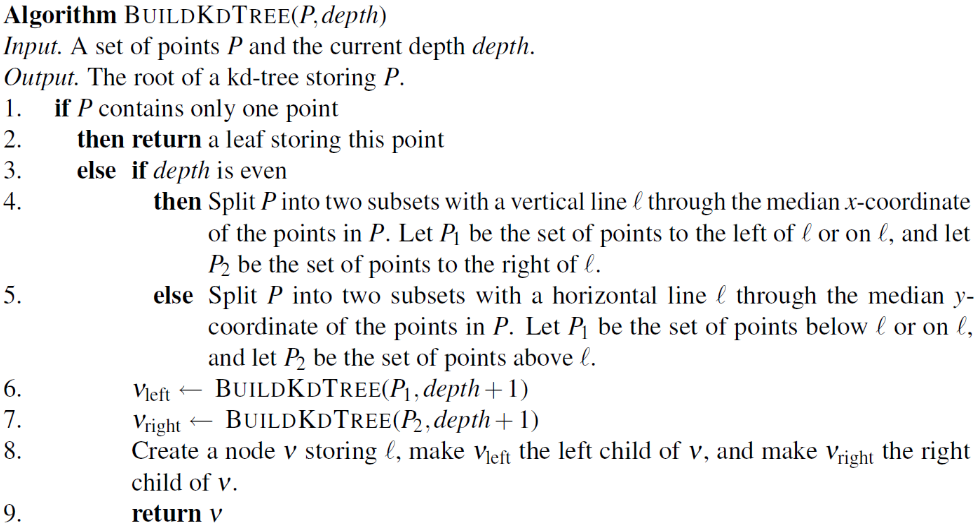
\includegraphics[width=0.7\linewidth]{afbeeldingen/kd-bomen/constructie}
			\label{fig:kd-constructie}
		\end{figure}
		Een kd-boom zal $O(n)$ aan geheugen nodig hebben en $O(n\log(n))$ aan tijdscomplexiteit. 
		\item[Zoeken]:\\
		Om te zoeken naar een interval, zal men de boom moeten aflopen. Elke knoop zal een extra grensniveau aanduiden en dus een kleinere regio definiëren. Hieronder volgen een goed visueel voorbeeld en de pseudocode voor dit algoritme. 
		\begin{figure}[h]
			\centering
			\subfigure{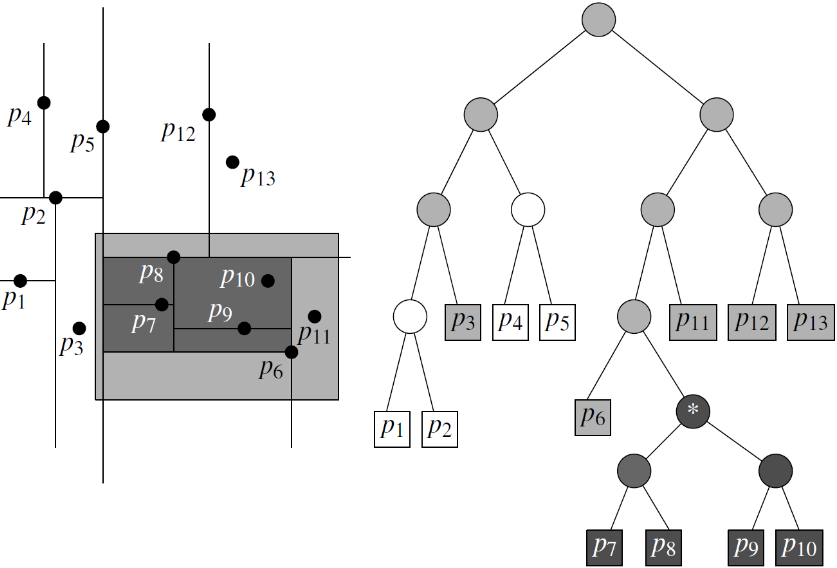
\includegraphics[width=0.40\textwidth]{afbeeldingen/kd-bomen/zoeken-voorbeeld}} 
			\subfigure{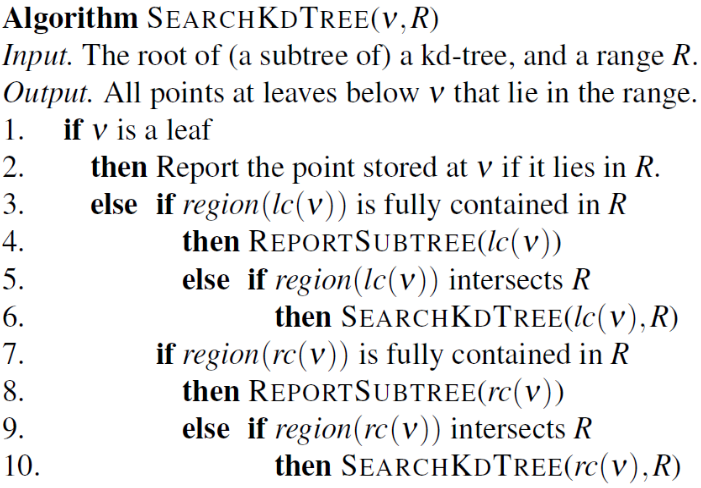
\includegraphics[width=0.40\textwidth]{afbeeldingen/kd-bomen/pseudocode}} 
			\label{fig:kd-zoeken}
		\end{figure}
		\item[efficiëntie]:\\
		Het rapporteren van de subbomen gebeurt in $O(k)$ met k het aantal punten dat teruggegeven moet worden als output. Het aantal knopen dat bezocht moet worden is $O(\sqrt{n})$. Deze expressie wordt gevonden door te kijken naar hoeveel regio's een horizontale lijn of een verticale lijn zou doorkruisen in zo'n regio in een kd-boom. Al deze doorsneden regio's vormen een boom met hoogte $\tfrac{1}{2}\log(n)$, aangezien we telkens twee grensniveaus moeten springen. Het totaal aantal regio's zal dan begrensd zijn door $2^{\frac{1}{2}\log(n)} = O(\sqrt{n})$. Zodra we beginnen aan hogere dimensies dan 2d, komen we aan een lineaire tijdscomplexiteit. 
	\end{description}
	
	
	\subsection{Range trees}
	Deze bomen zijn eigenlijk gelijk aan de kd-bomen, enkel dat ze snellere zoektijd willen bekomen ten koste van het geheugen. 
	
	Voor 1d houdt een range tree in: Vanaf een split node kunnen we opslaan wat de mogelijke eindknopen zijn van de zoekopdracht. 
	
	Voor 2d zal er een gebalanceerde boom zijn op basis van de x-coordinaat, in elke knoop is dan een nieuwe gebelanceerde boom op basis van de y-coordinaat. 
	
	Voor grotere dimensies voel je aan dat er dan per knoop nog extra dimensies zullen volgen. Elk punt zal maximaal 1 keer opgeslagen zijn in de boom $\rightarrow O(n)$ per niveau. Per punt zijn er dan $P(\log(n))$ niveaus  waarop het punt wordt opgeslagen. Het geheugen zal hier dus $O(n\log(n))$ zijn. De pseudocode voor het opbouwen en het zoeken zijn hieronder gegeven: 
	\begin{figure}[H]
		\centering
		\subfigure{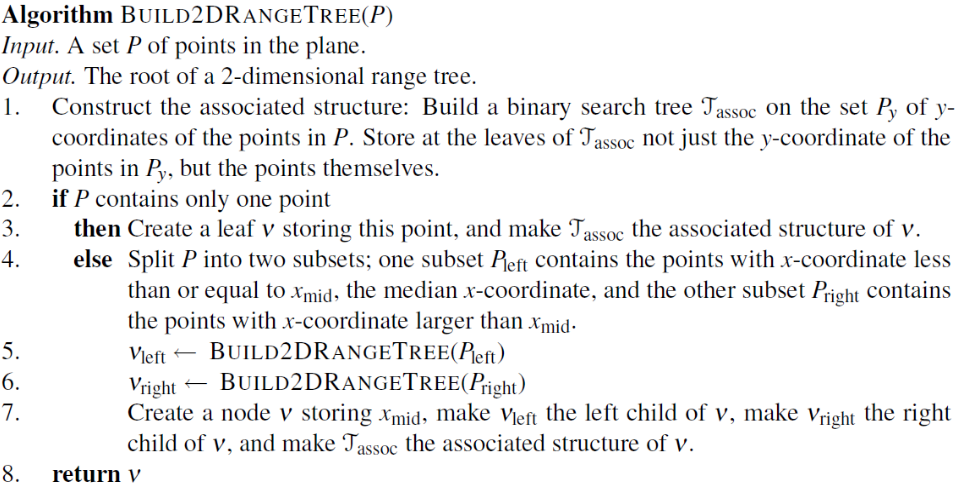
\includegraphics[width=0.49\textwidth]{afbeeldingen/kd-bomen/rangetree-build}} 
		\subfigure{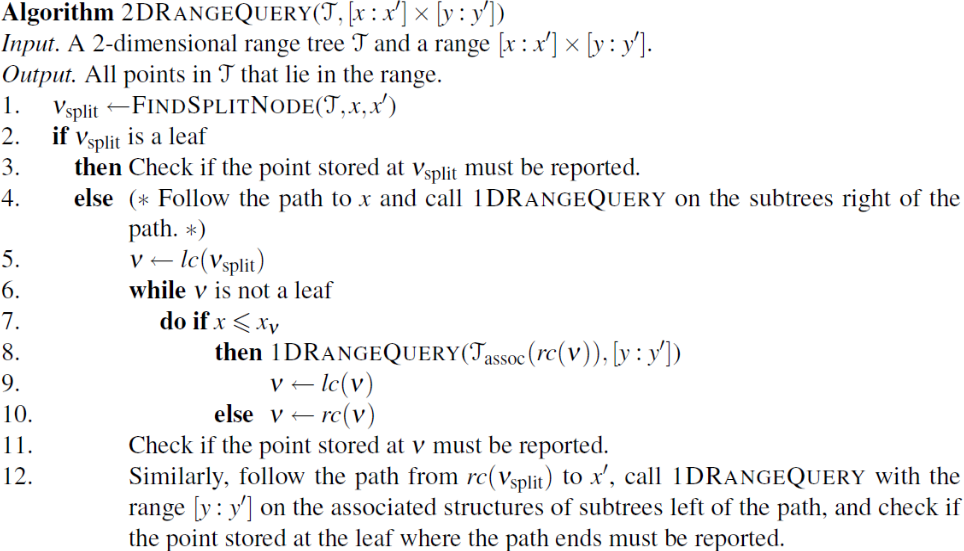
\includegraphics[width=0.49\textwidth]{afbeeldingen/kd-bomen/rangetree-zoeken}} 
		\label{fig:range-treees-pseudocode}
	\end{figure}

	De tijdscomplexiteit bij range zal inderdaad beteren, zoals hieronder te zien: 
	
	\begin{figure}[H]
		\centering
		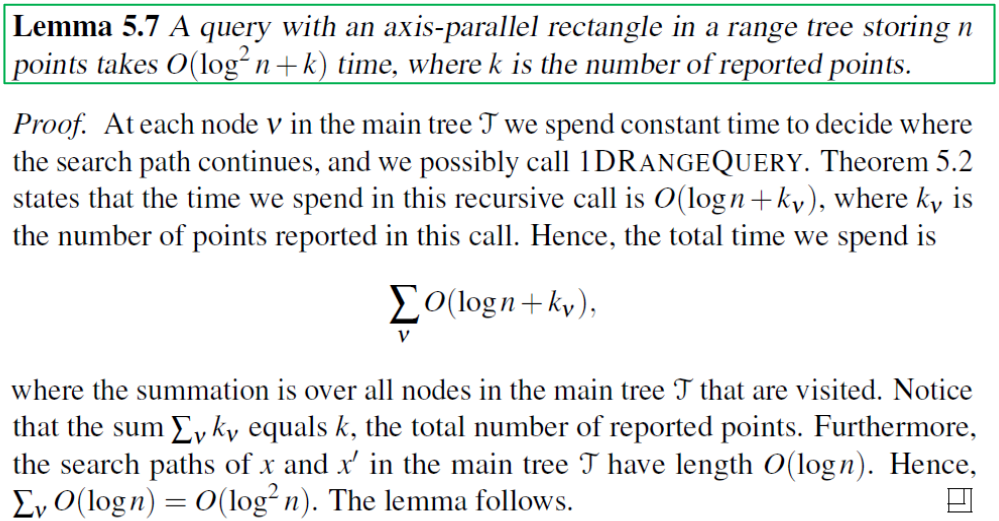
\includegraphics[width=0.7\linewidth]{afbeeldingen/kd-bomen/rangetrees-tijdscomplexiteit}
		\label{fig:rangetrees-tijdscomplexiteit}
	\end{figure}
	 
	
	
	\subsection{Typische examenvragen}
	\begin{itemize}
		\item \textbf{Wat is een kd-boom? Leg uit:}\\
		\item \textbf{Wat is de tijdscomplexiteit voor het opzoeken van alle punten binnen een (gegeven) 2D-interval in een tweedimensionale kd-boom?:}\\
		\item \textbf{Leg de idee uit van Range Trees:}\\
	\end{itemize}
	
	%TODO hier zit ik!
	\section{Puntlocatie}
	Deze les is gebaseerd op de vraag: ligt een punt in een gegeven veelhoek? 
	
	
	\subsection{Een aantal oplossingen}
	In dit deel worden een aantal oplossingen overlopen, allemaal heel simpel maar niet perse heel efficiënt. 
	\begin{itemize}
		\item We kunnen vanaf het punt kijken hoeveel snijpunten deze heeft met de veelhoek, als dit oneven is zal het punt in de veelhoek liggen. En probleem hiermee is wat al men hoekpunten tegenkomen? Dit is een edge case maar is wel heel relevant. 
		\item Een andere manier is de som te nemen van alle hoeken met alle hoekpunten van de veelhoek. Als de som van deze hoeken 0° is, dan is het punt buiten de veelhoek. Als de som 360° is, dan zit het punt wel in de veelhoek.
		\item Er is ook een manier om dit te bepalen met de kwadranten van een assenstelsel, waarbij er bijgeteld moet worden of niet bij het veranderen van een kwadrant. 
		\item Er kan een grid worden geplaatst over de veelhoek, afhankelijk van in wekl vierkantje het punt ligt weten we al op voorhand of het in de veelhoek zit of niet. In de vierkantjes kan ook een zijde van de veelhoek liggen, dan moeten er meer testen volgen. 
	\end{itemize}
	
	\subsection{Vlakverdeling}
	Een eerste aanpak tot het verdelen van de ruimte in verticale stroken die liggen op punten waar lijnen snijden. Het geheugencomplexiteit is dan $2n$, terwijl de tijdscomplexiteit om een punt te bepalen binnen een slab query $O(\log(n))$ is. Binnen zo een slab snijden er geen edges, deze kunnen dus gesorteerd worden op basis van y-coördinaat, elke slab heeft een $O(n)$ geheugen nodig. Het vinden van de locatie binnen de slab zal dus $O(\log(n))$ vragen. Het totale geheugen zal dus $O(n^2)$ vragen, wat niet ideaal is. 
	\\
	\\
	Een tweede aanpak is een \textit{trapezium map} opstellen van de vlakverdeling. Hier verbinden we elke vertex met de edge erboven en erronder. We veronderstellen hier dat elke vertex een verschillend x-coördinaat heeft en dat er een bounding box bestaat rond de vlakverdeling. De faces die zullen overblijven, zijn allemaal driekhoeken of trapezia. Deze trapezia zullen bepaald worden door: \textit{top, bottom, leftp, rightp}, top en bottom verwijzen naar edges en leftp en rightp verwijzen naar trapezia. Over deze trapezium map bestaat ook nog een lemma: 
	\begin{figure}[H]
		\centering
		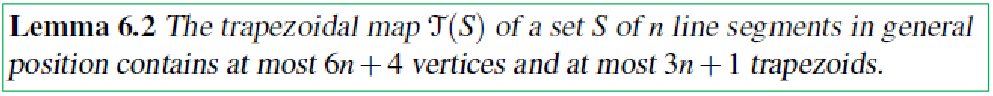
\includegraphics[width=0.9\linewidth]{afbeeldingen/trapezium-map/lemma}
		\label{fig:lemma}
	\end{figure}
	
	S zal bestaan uit $2n$ vertices, waarbij elke vertex 2 nieuwe vertices kan creëeren. De bounding box zelf bevat nog eens 4 vertices, wat een totaal geeft van $\rightarrow 4 + 2n + 2(2n) = 6n + 4$ vertices. Het links eindpunt van een segment kan een linkerzijde van 2 trapezia definiëren, een rechts eindpunt kan een linkerzijde van 1 trapezium definiëren. R definieerd del linkerzijde van 1 trapezium, diet komt neer op $3n + 1$ trapezia. Twee trapezia die aangrenzend zijn (dus een verticale lijn gemeenschappelijk) hebben altijd een top of bottom gemeenschappelijk. Elk lijnsegment zal in deze structuur verwijzen naar 2 eindpunten en de oorspronkelijke face die boven de edge ligt. Een trapezium kan dus via bottom te weten komen in welke face deze zit. 
	
	De effectieve gegevensstructuur die hiervoor kan gebruikt worden is een gerichte acyclische graaf (DAG). Elk blad is dan een trapezium, de x-knopen zijn de eindpunten van segmenten, deze verwijzen dan naar een lijnsegment (de y-knopen) die dan een boven en onder test hebben die verwijzen naar de trapezia. Het opstellen van deze graaf zal verlopen via een RIC (Randomized Incremental Constitution), zoals in de vorige les gezien. 
	Er zal dus telkens een nieuw lijnsegment worden toegevoegd en hier zal dus de trapezium map rond aangepast worden. Deze aanpasseingen gaan heel plaatselijk zijn, waardoor het RIC dus heel erg handig is. Het toevoegen van een lijnsegment zal twee stappen ondervinden:  
	\begin{enumerate}
		\item Als eerste overlopen we het nieuwe toegevoegde lijnstuk en duiden we alle trapezia waar die lijnstuk door ligt. Dit door telkens te zoeken naar bovenliggende lijnstukken, waarbij we het linkereindpunt zoeken en van daaruit kijken naar de trapezia. Hieronder volgt de pseudocode, voor een duidelijk visuele representatie: check de slides ;). 
		\begin{figure}[H]
			\centering
			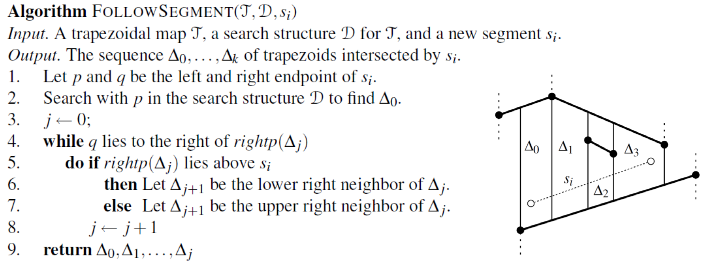
\includegraphics[width=0.7\linewidth]{afbeeldingen/trapezium-map/stap1-lijnstukken}
			\label{fig:stap1-lijnstukken}
		\end{figure}
		
		%TODO herbekijken in de les. 
		\item Als tweede zullen we de verticale verdeling updaten. In het algemene geval zal de graaf dan geüpdated moeten worden vanaf een bepaald niveau in de boom, en vraagt die niet ontzettend veel rekenwerk. 
	\end{enumerate}
	De tijdscomplexiteit van de eerste stap is het zoeken van k trapezia. $O(k)$. Dit is ook de comlexiteit van de tweede stap voor het aantal interne knopen en het aantal bladeren. 
	\\
	!! Examenvraag !!: Zo'n graaf kunnen opstellen voor een aantal lijnsegmenten, les opnieuw bekijken en snappen!!!
	
	De uiteindelijke trapezium zal niet afhangen van de RIC, maar de uiteindelijke graaf wel! Zo kan het zijn dat een graaf heel efficiënt is of net helemaal niet. Voor de analyse van de tijdscomplexiteit, kijken we naar de uitkomst want ik ben effe te moe om dit na te kijken en moet de les best herbekijken hiervoor. 
	\begin{figure}[H]
		\centering
		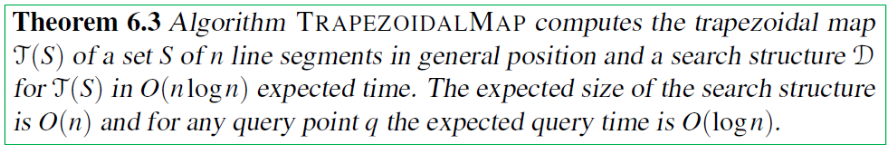
\includegraphics[width=0.9\linewidth]{afbeeldingen/trapezium-map/theorem}
		\label{fig:theorem}
	\end{figure}
	
	
	\subsection{Typische examenvragen}
	\begin{itemize}
		\item \textbf{Leg de pincipes uit van een trapezium-map:}\\
		\item \textbf{Leg het algoritme uit om een lijnsegment toe te voegen aan een bestaande trapezium-map:}\\
		\item \textbf{Op welke manieren kunnen we nagaan of een punt behoort tot het inwendige van een veelhoek?:}\\
	\end{itemize}
	
	
	\section{Voronoi Diagramma's}
	Gegeven een verzameling 'sites' (of gewoon punten op een vlak), wat is de meest nabije site voor om het even welk punt in het vlak. De terminologie is hieronder nog eens te lezen: 
	\begin{figure}[H]
		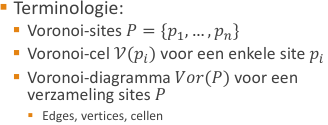
\includegraphics[width=0.4\linewidth]{afbeeldingen/voronoi/terminologei}
		\label{fig:terminologei}
	\end{figure}
	
	
	\subsection{Enkele observaties}
	Het valt op dat in deze diagrammen, de edges telkens de middelloodlijn zijn tussen de 2 sites. Niet alle edges zijn begrensd, wat dus ook uitbreid tot dat niet elke voronoi-cel begrensd is. De edges zullen elk samenkomen in een vertex, de voronoi-vertex. 
	
	Elke voronoi-vertex is de doorsnede van $n-1$ halfvlakken, wat betekent dat elke cel convex is en door tot $n-1$ edges kan bergensd zijn. De structuur van zo'n voronoi diagramma kan in een stelling worden geschreven en ook bewezen: 
	\begin{figure}[H]
		\centering
		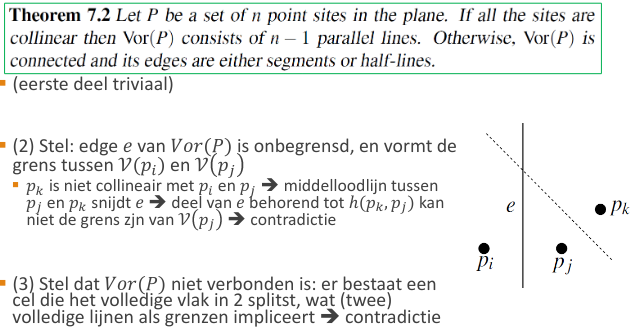
\includegraphics[width=0.8\linewidth]{afbeeldingen/voronoi/structuur}
		\label{fig:structuur}
	\end{figure}
	
	De tijdscomplexiteit kan ook afgeleid worden uit het aantal sites, het aantal vertices en het aantal edges: 
	\begin{figure}[H]
		\centering
		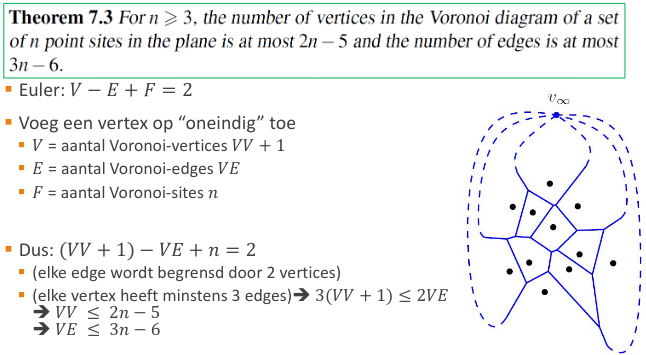
\includegraphics[width=0.8\linewidth]{afbeeldingen/voronoi/complexiteit}
		\label{fig:complexiteit}
	\end{figure}
	
	
	Naast deze observaties, structuren en complexiteit zijn er ook een aantal eigenshappen die bij voronoi diagramma's gelden, meer specifiek eigenschappen met cirkels: 
	
	\begin{itemize}
		\item Elke voronoi-vertex is het centrum van een cirkel door 3 voronoi-sites. 
		\item Elk punt op een voronoi-edge is het centrum van een cirkel door 2 sites.
	\end{itemize}
	
	Na al deze uitbundige informatie, komen de algoritmes om zo een voronoi-diagramma te bepalen. 
	
	\subsection{Algoritmes}
	\begin{description}
		\item Een eerste manier is om te werken met dat een voronoi-veelhoek gezien kan worden als de doorsnede van $n-1$ halfvlakken. 
		\item[Incrementeel algoritme]: Telkens een nieuwe site toevoegen aan het voronoi diagramma, er wordt dan met de cirkeleigenschappen bekken welke voronoi-edges opnieuw berekend moeten worden. 
		\item[Verdeel-en-heers algoritme]: Eerst een deel van de sites verwerken en het diagramma opstellen om dan te mergen. 
		\item[Doorlooplijn]: De doorlooplijn zou over de sites als events lopen en op die manier het diagramma aanpassen, het probleem hierbij is dat een doorlooplijn niets kan aanpassen aan waar die al is langsgeweest. Dit kan een probleem maken aangezien de edges achter de doorlooplijn wel nog kunnen veranderen. 
		\item[Groeiende cirkels]: De voronoi cellen zijn cirkels die vanuit een site starten om groter te worden en uiteindelijk de voronoi edges te bepalen. Hieronder volgt een visualisatie: 
		\begin{figure}[h]
			\centering
			\subfigure{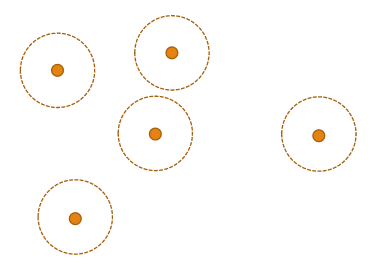
\includegraphics[width=0.32\textwidth]{afbeeldingen/voronoi/groeiende-cirkels-first}} 
			\subfigure{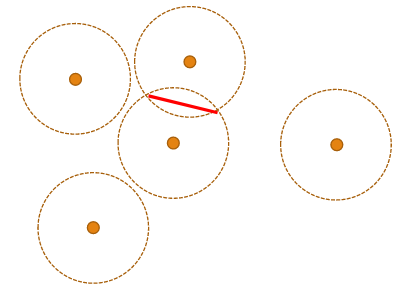
\includegraphics[width=0.32\textwidth]{afbeeldingen/voronoi/groeiende-cirkels-second}} 
			\subfigure{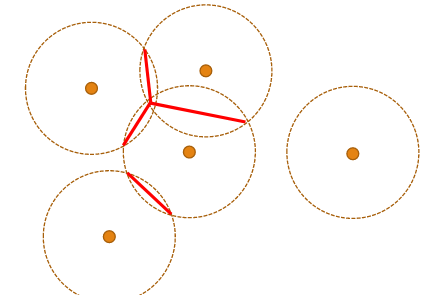
\includegraphics[width=0.32\textwidth]{afbeeldingen/voronoi/groeiende-cirkels-third}}
			\label{fig:groeiende-cirkels-voorbeeld}
		\end{figure}
		\item[Groeiende kegels]: Hetzelfde concept als de cirkels maar er is nu ook de tijdsmeting op de z-as. Het uiteindelijke resultaat wordt dan op het xy-vlak geprojecteerd. 
		\item[Doorloopvlak]: Een vlak dat schuin staat tegenover het xy-vlak, onder dezelfde hoek als de kegels (van hierboven). De snijding met de kegel maakt dan een golf na en alles achter die golf kan niet meer aangepast worden. Dit is de basis voor het meest efficiënte algoritme dat in het deel hieronder besproken zal worden. 
	\end{description}
	
	
	\subsection{Het golffront}
	Het golffront is de projectie van de parabolische snijding op het xy-vlak van de kegel met het schuin doorloopvlak. Deze projectie vormt een parabool op het vlak. Telkens als deze doorlooplijn een nieuwe site tegenkomt, zal een nieuwe parabool deel worden van het golffront. Hieronder vind je nog een visualisatie van zo'n golffront met een afbeelding die toont hoe de parabool wordt gemaakt. 
	\begin{figure}[H]
		\centering
		\subfigure{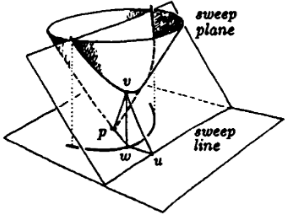
\includegraphics[width=0.39\textwidth]{afbeeldingen/voronoi/golffront-parabool}} 
		\subfigure{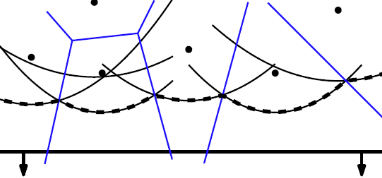
\includegraphics[width=0.59\textwidth]{afbeeldingen/voronoi/golffront-front}} 
		\label{fig:golffrront-parabool}
	\end{figure}
	
	Zoals hierboven zichtbaar, zal ekle site zo een parabool bepalen, de theorie achter zo'n parabool is dat die nooit dichter bij een site onder de doorlooplijn kan zitten dan bij de site die de parabool maakt. Het golffront scheidt het gekende en het ongekende deel van het Voronoi-diagramma en wijzigt ook naarmate de doorlooplijn vordert. 
	
	Het is ook zichtbaar dat de breekpunten (snijpunt tussen twee parabolen) een voronoi-edge bepalen. Voor dit algoritme zullen ook een aantal belangrijke concepten besproken worden: 
	
	\begin{description}
		\item[Status golffront]: Gesorteerde sequentie vqn paraboolsegmenten: Breekpunten knopen, sites bladeren. 
		\item[Event queue]: Doorlooplijn stopt bij een nieuwe voronoi-site en wanneer een breekpunt het einde van een voronoi-edge bereikt. 
		\item[Site event]: Wanneer de doorlooplijn een site tegenkomt, zal deze een nieuwe parabool toevoegen aan het golffront, dit gaat aanvankelijk een verticale lijn zijn maar zal breder worden naarmate de doorlooplijn vordert. De twee nieuwe breekpunten die deze site veroorzaken zullen op dezelfde locatie starten en dan van mekaar weg bewegen. Voor duidelijkheid volgt een visualisatie: 
		\begin{figure}[H]
			\centering
			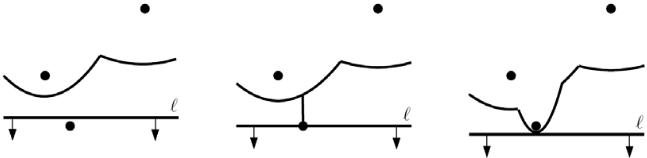
\includegraphics[width=0.7\linewidth]{afbeeldingen/voronoi/site-event}
			\label{fig:site-event}
		\end{figure}
	
		Het golffront zal ten allen tijde maximaal uit $2n-1$ paraboolsegmenten bestaan. Dit komt omdat er maar zoveel parabolen kunnen zijn als site-events en dat door het toevoegen van een paraboolsegment, een ander segment in 2 kan worden gesplitst. Hier komt de $2n$ dus natuurlijk vandaan. De -1 is aangezien dat er altijd een segment zal zijn dat niet in 2 is gedeeld, gezien dat dat net andere segmenten in twee heeft gedeeld. Hieronder volgt de pseudovode voor dit algoritme: 
		\begin{figure}[H]
			\centering
			\includegraphics[width=0.8\linewidth]{afbeeldingen/voronoi/handleSiteEvent}
			\label{fig:handlesiteevent}
		\end{figure}
		
		\item[Cirkel-event]: Dit event wordt getriggered wanneer er twee breekpunten samenkomen. Op het moment dat ze samenkomen zal een cirkel gevormd worden met 3 sites op de rand. De cirkel moet op dat moment ook de doorlooplijn raken en moet ook leeg zijn (er mogen geen voronoi sites inzitten die bijvoorbeeld onder de doorlooplijn liggen). Het centrum van die cirkel is dan de voronoi-vertex en dan zal het golffront als breekpunt van twee paraboolsegmenten verdergaan. Dit event is de enige manier om een paraboolsegment te laten verdwijnen. Hieronder volgt een visualisatie: 
		\begin{figure}[H]
			\centering
			\includegraphics[width=0.7\linewidth]{afbeeldingen/voronoi/cirkel-event}
			\label{fig:cirkel-event}
		\end{figure}
		Het bepalen van deze cirkels lijkt een vrij moeilijk gegeven, om het te versimpelen kan er voor elk trio aan buren bijgehouden worden wat de cirkel is die zij definiëren. Dit betekent niet dat elk van deze cirkels een cirkel-event zal trigeren, sommigen kunnen namelijk een 'false alarm' zijn. Het onderste deel van de cirkel kan dan ook een event zijn om na te kijken of deze cirkel geldig is en effectief een voronoi-vertex definieert. Ook hier hoort pseudocode bij: 
		\begin{figure}[H]
			\centering
			\includegraphics[width=0.8\linewidth]{afbeeldingen/voronoi/handeCircleEvent}
			\label{fig:handecircleevent}
		\end{figure}
		
	\end{description}
	De constructie van het voronoit diagramma zal dus bestaan uit een golffront dat uitgebreid wordt als een site bereikt wordt en ingekrompen wordt als een cirkel-event plaatsvindt. 
	
	Voor dit algoritme zullen ook een aantal datastructuren nodig zijn: 
	\begin{description}
		\item - Het voronoi-diagramma zal gemaakt worden uit een DCEL. 
		\item - De event queue moet bestaan uit een gesorteerde lijst site-events. De cirkels moeten gedetecteerd worden voor 3 opeenvolgende paraboolsegmenten. Dit betekent niet dat elk trio een bruikbare cirkel definiëren. Telkens een site-event plaatsvindt zijn er 3 mogelijke nieuwe tio's voor de cirkel: een links, een midden en een rechts. Als dit tripel aanleiding geeft tot een cirkel event wordt dit toegevoegd aan de event queue. 
		\item - Het golffront zelf moet bestaan uit een gebalanceerde zoekboom. Hier zijn de bladeren de paraboolsegementen (van links naar rechts in de boom) en elk blad bevat ook de site waarbij dat segment hoort. De interne knopen van de boom zijn de breekpunten $\rightarrow$ Gegeven een nieuw site-event kunnen we gemakkelijk in $\log(n)$ tijd het paraboolsegment vinden dat boven deze nieuwe site ligt. 
	\end{description}
	Hieronder volgt de code voor de constructie nog, met een oproep naar HandleSiteEvent en een oproep naar HandleCircleEvent. 
	\begin{figure}[H]
		\centering
		\includegraphics[width=0.9\linewidth]{afbeeldingen/voronoi/voronoi-diagramma}
		\label{fig:voronoi-diagramma}
	\end{figure}

	De operaties op het golffront zullen elk $O(\log(n))$ hebben als tijdscomplexiteit. Er zijn $n$ site-events en maximaal $2n-5$ cirkel-events. De totale complexiteit zal dus uiteindelijk $O(n\log(n))$ zijn. 
	
	
	\subsection{Verdere uitbreidingen}
	\begin{description}
		\item[Diagram van lijnsegmenten]: De edges zijn da lijnsegmenten of paraboolsegmenten en we veronderstellen voor dit algoritme geen samenvallende punten. Het algoritme zal heel erg analoog zijn, er zullen gewoon meer scenario's zijn bij breekpunten. 
		\item[Toepassing: padplanning]: Een robot kan zich verplaatsten volgens de voronoi-edges en zal zo niet botsen met de sites/obstakels. 
		\item[Hogere orde diagrammen]: Er bestaan ook hogere orde diagrammen. Een 2e orde is bijvoorbeeld de twee dichtstbijzijnde buren voor een bepaald punt in de ruimte. Deze orde kan groter en groter worden tot de $n-1$ste orde (met n het aantal sites). Deze laatste wordt ook wel het \textit{verste punt diagramma} genoemd, gezien het dan kijken naar wat het verste ligt voor een punt. Alle cellen van dit diagram zullen onbegrensd zijn. Het opstellen van deze constructie moet incrementeel gebeuren. Een mooie visualisatie hiervan:
		\begin{figure}[H]
			\centering
			\includegraphics[width=0.9\linewidth]{afbeeldingen/voronoi/hogere-orde}
			\label{fig:hogere-orde}
		\end{figure}
		
		Er volgt dan ook nog een klein voorbeeld waarbij naarmate je andere functies voor de afstand kiest, je diagram er anders kan uitzien.
	\end{description} 
	
	
	\subsection{Typische examenvragen}
	\begin{itemize}
		\item \textbf{Wat is het verband tussen het Voronoidiagramma van een verzameling punten, en de Delaunay triangulatie?:}\\
		\item \textbf{Leg het sweep-line algoritme van Fortune uit om een Voronoidiagramma te construeren:}\\
		\item \textbf{Bewijs eigenschap X van Voronoi-diagramma's. Welk belang heeft deze eigenschap voor de algoritmische constructie van Voronoi-diagramma's?:}\\
		\item \textbf{De Voronoi-veelhoek behorend bij een punt p dat behoort tot S is begrensd als en slechts als p behoort tot het inwendige van de convex omhullende van S. Bewijs deze eigenschap. Waar wordt deze eigenschap gebruikt, of waarom is ze nuttig?:}\\
		\item \textbf{Hoe bewijs je dat een Voronoi-diagram van een verzameling van N sites maximaal 2N-5 Voronoi-punten en maximaal 3N-6 Voronoi-zijden bezit? Waarom is het belangrijk dat het aantal Voronoi-zijden (slechts) O(N) is? Geef minstens één voorbeeld van het nut van deze eigenschap:}\\
		\item \textbf{(Gegeven een tekening met een aantal punten als Voronoi-sites en een positie van de doorlooplijn). Schets op bijhorende tekening het golffront voor de positie die de doorlooplijn reeds bereikt heeft, teken eveneens de Voronoi-punten en Voronoi-zijden die het algoritme van Fortune reeds bepaald heeft. Schrijf eventueel commentaar bij je tekening om één en ander te verduidelijken:}\\
		\item \textbf{Geef een voorbeeld waarbij de parabool behorende bij een Voronoi-site méér dan 1 segment bijdraagt aan het golffront (algoritme van Fortune):}\\
		\item \textbf{Geef een voorbeeld waarbij voor 6 Voronoi-sites, elk van de 6 sites door de doorlooplijn behandeld worden, vooraleer er een cirkel-event plaatsvindt. De sites moeten algemeen van aard zijn, ttz geen 3 sites op een lijn of 4 sites op een cirkel:}\\
	\end{itemize}
	
	
	\section{Delaunay Triangulatie}
	Deze triangulaties komen uit het probleem: hoe interpoleer je de hoogte van een punt tegenover de omliggende punten. Een naïve manier om dit op te lossen is door een voronoi-diagram te maken en voor elke cel is de hoogte van die cel gelijk aan de hoogte van de site. Een andere manier is om voor elk punt de gemiddelde hoogte van de buren te pakken. Je voelt onmiddelijk aan dat deze technieken niet altijd een correct beeld zullen geven van een 3D terrein. Een betere oplossing is door de ruimte te trianguleren tussen de punten en er lineaire interpolatie bij toe te passen. 
	
	Een triangulatie is niet eenduidig bepaald en er zijn dus logish triangulaties die beter geschikt zijn dan anderen. Een goede manier om een goede triangulatie te bepalen is bijvoorbeeld zeggen dat de lengte van de zijdes van de driehoek even lang moeten zijn (of zo gelijk mogelijk) of dat de hoeken allemaal zo dicht mogelijk bij 60°. Dit is allemaal heel 'hard-coded' en zou niet altijd het meest efficient kunnen zijn. Een vaste regel kan dus zijn: \textit{De minimale hoek van alle driehoeken moet gemaximaliseerd zijn.}
	
	
	\subsection{Triangulatie van een puntenset}
	De triangulatie van punten is \textit{the maximal planar subdivision}. Triangulaties hebben een aantal eigenschappen: 
	\begin{itemize}
		\item Er kunnen geen edges meer toegevoegd worden zonder andere edges te snijden. 
		\item Veelhoeken kunnen telkens verder gesplitst worden in driehoeken
		\item De edges van de convex imhullende zijn steeds deel van de triangulatie.
	\end{itemize}

	Deze triangulaties zullen altijd $2n - 2 - k$ driehoeken hebben met $n$ het aantal punten en met $k$ het aantal punten op de convex omhullende. Ze zullen ook altijd $3n - 3 - k$ edges hebben met dezelfde parameters. Het bewijs kan gemakkelijk gevonden worden aan de hand van de formule van Euler. 
	
	Stel $T(p)$ een triangulatie van p met m driehoeken, de \textit{Angle vector} $A(T)$ waarbij het een vector is met de hoeken van die triangulatie gesorteerd van klein naar groot. Stel dan een andere triangulatie voor $T'(p)$. $T(p)$ is de \textit{angle optimal} wanneer voor alle alternatieve $T'(p)$ geldt dat: $A(T) > A(T')$. Een triangulatie kan geoptimalisseerd worden door een edge flip uit te voeren, zoals hieronder te zien is: 
	\begin{figure}[H]
		\centering
		\includegraphics[width=0.9\linewidth]{afbeeldingen/delaunay/edge-flip}
		\label{fig:edge-flip}
	\end{figure}

	Zo'n edge flip wordt gebruikt wanneer door het wisselen van een edge, de Angle vector optimaler kan worden. Een edge is dus illegaal wanneer de angle vector van een alternatieve triangulatie beter is dan de huidig en dit door een edge flip gebeterd kan worden. Een illegale edge kan gedetecteerd worden door middel van en eigenschap met cirkels. De eigenschap staat hieronder geïllustreerd met een voorbeeld: 
	\begin{figure}[H]
		\centering
		\subfigure{\includegraphics[width=0.47\textwidth]{afbeeldingen/delaunay/illegal-edge}} 
		\subfigure{\includegraphics[width=0.51\textwidth]{afbeeldingen/delaunay/illegal-edge2}} 
		\label{fig:illegal-edges}
	\end{figure}

	Het berekenen van een legale triangulatie zal als volgt verlopen: 
	\begin{figure}[H]
		\centering
		\includegraphics[width=0.7\linewidth]{afbeeldingen/delaunay/legalTranslation}
		\label{fig:legaltranslation}
	\end{figure}

	Dit algoritme zal ook eindigen: er is een eindig aantal triangulaties, therefore een eindig aantal keer dat dit algoritme kan lopen om alle illegale edges te verwijderen. 
	
	
	\subsection{Delaunay triangulaties}
	Deze triangulatie zal eerst het voronoi diagram opstellen van de punten waarmee de triangulatie gemaakt moet worden. Dan wordt de duale graaf gemaakt van dit diagram met als edges telkens de connectie tussen twee buren in het voronoi diagram. De \textit{Delaunay} is dan het gebruik maken van die duale graaf door er rechte lijnen van de maken. Het is dan ook duidelijk uit deze constructie dat de Delaunay graaf een vlakke graaf zal zijn (er zijn geen edges die elkaar snijden), dit is af te leiden uit een van de eigenschappen van het voronoi deel. Hier volgen een aantal eigenschappen waarvoor ik te lui ben om ze op te schrijven B): 
	
	\begin{figure}[H]
		\centering
		\subfigure{\includegraphics[width=0.49\textwidth]{afbeeldingen/delaunay/theorem1}} 
		\subfigure{\includegraphics[width=0.49\textwidth]{afbeeldingen/delaunay/theorem2}} 
		\subfigure{\includegraphics[width=0.49\textwidth]{afbeeldingen/delaunay/theorem3}} 
		\subfigure{\includegraphics[width=0.49\textwidth]{afbeeldingen/delaunay/theorem4}} 
		\label{fig:delaunay-theorems}
	\end{figure}
	\begin{description}
		\item[Constructie]: Hier zijn ook weer een aantal opties, maar uiteindelijk zal een RIC zorgen voor een efficiënt algoritme. Het toevoegen van een nieuw punt zal maar lokaal veranderingen veroorzaken, wat dus logisch lijkt te leiden tot een kleine tijdscomplexiteit. 
		
		Het algoritme begint met het verbinden van de drie punten die (als verbonden) in hun driehoek alle andere punten omvat. Na deze stap kunnen er twee soorten toevoegingen gebeuren: ofwel wordt een puntin een driehoek toegevoegd, ofwel wordt een punt toegevoegd dat op een edge ligt. In het eerste geval moeten er edges naar de vertices van deze driehoek getrokken worden en in het tweede geval moeten er twee edges naar de uiterste vertices getrokken worden. Na deze operatie moet ter plekke telkens nagekeken worden of de triangulatie legaal is. De pseudocode kan je hieronder vinden: 
		\begin{figure}[H]
			\centering
			\subfigure{\includegraphics[width=0.49\textwidth]{afbeeldingen/delaunay/delaunayTriangulatie1}} 
			\subfigure{\includegraphics[width=0.49\textwidth]{afbeeldingen/delaunay/delaunayTriangulatie2}} 
			\subfigure{\includegraphics[width=0.50\textwidth]{afbeeldingen/delaunay/legalizeEdge}} 
			\label{fig:delaunay-constructie}
		\end{figure}
		
		Hoe weten we nu in welke driehoek een punt ligt? Dit kunnen we doen door een zoekstructuur (een soort graaf bijvoorbeeld). Een ander probleem is de eerste drie punten bepalen. We kunnen ook zelf twee punten 'uitvinden' die ver genoeg liggen en telkens deze punten betrokken zijn ervoor zorgen dat deze niet in de triangulatie komen. Op die manier bekomen we wel nog een correct resultaat. 
		
		\item[Analyse]: 
		De afleiding voor deze tijd en ruimte complexiteit moeten we (YES) niet kennen! Het geheugen zal als complexiteit $O(n)$ hebben. De uitvoeringstijd van een puntlocatiestap hangt af van hoeveel driehoeken we moeten overlopen om te vinden waar het punt ligt en per driehoek moet dan bepaald worden hoeveel punten in de omhullende cirkel liggen. Uiteindelijk komen we uit op, het alomgekende: $O(n\log(n))$. 
	\end{description}
	
	Voor dit algoritme zijn er natuurlijk een aantal toepassingen, zoals ray tracing (cool ze). 
	
	
	\subsection{Typische examenvragen}
	\begin{itemize}
		\item \textbf{Leg het verband uit tussen het Voronoi-diagramma van een puntenset en de Delaunay triangulatie van diezelfde puntenset:}\\
		\item \textbf{Op welke manier kan de Delaunay-triangulatie van een puntenset geconstrueerd worden?:}\\
		\item \textbf{Leg de equivalentie uit tussen de "cirkeleigenschappen" in zowel het Voronoi-diagramma als de Delaunay-triangulatie:}\\
		\item \textbf{Gegeven een set punten met bijhorende triangulatie. Is de getekende triangulatie een Delaunay-triangulatie? Waarom wel? Waarom niet? Welke eigenschappen kan je gebruiken om dit vast te stellen?:}\\
		\item \textbf{In een getekende Delaunay-triangulatie wordt een punt toegevoegd. Schets de resulterende Delaunay-tiangulatie:}\\
	\end{itemize}
	%Opmerking: vragen waarbij gevraagd wordt handmatig na te gaan of bepaalde eigenschappen gelden in een getekende Delaunay-triangulatie of Voronoi-diagramma zullen natuurlijk geen "milimeter-werk" zijn om iedereen op stang te jagen. Vaak zou je de cirkeleigenschappen met het blote oog moeten kunnen zien of gemakkelijk moeten kunnen afleiden met een eenvoudige construtie met een meetlat of passer ...
	
	
	\section{Béziercurven}
	Dit deel is gebaseerd op te zoeken naar een curve dat een aantal punten volgt. 
	
	
	\subsection{Interpolerende veeltermcurven}
	Deze veeltermcurve zal gegeven n+1 punten een curve maken voor de punten p met als parameterwaarde u (gaande van 0 tot n). De curve zal dus afhankelijk zijn van alle punten en een kleine wijziging zal heel de curve aanpassen. Dit is in het algemeen nadelig aangezien de curves plaatselijk aanpassen wel een handige tool is. De curve volt ook de punten niet volledig, het is heel uiteenlopend. Het is duidelijk dat dit niet echt fantastisch is. 
	
	
	\subsection{Lagrange veeltermen}
	Deze veelterm gaat zich baseren op de veeltermcurve en zal bestaan uit volgende vergelijking: 
	\[L_i^n(u) = \prod_{k = 0, k \neq i}^{n} \frac{u - u_k}{u_i - u_k}, 0 \leq i \leq n\]
	Met i de 'i-de' Lagrangeveelterm van de n-de graad. Hier volgen ook een aantal eigenschappen bij: 
	\[L_i^n(u_i) = 1, L_i^i(u_j) = 0, j \neq i\]
	\[\sum_{k = 0}^{n} L_k^n(u) = 1, \forall u \in [u_0, u_n]\]
	
	Er volgt ook nog een visualisatie om te snappen wat die eigenschappen inhouden: 
	\begin{figure}[H]
		\centering
		\includegraphics[width=0.8\linewidth]{afbeeldingen/Beziercurven/Lagrange-veelterm-voorbeeld}
		\label{fig:lagrange-veelterm-voorbeeld}
	\end{figure}

	Een gevolg van deze eigenschappen: 
	\[\sum_{k = 0}^{n} x_k L_k^n(u_i) = x_i\]
	Waarbij alle 'u-waarden' gelijk zijn aan 0. Met dit gevolg kan het verloop volgens de x-as en de y-as dan gemaakt worden. 
	
	We kunnen deze curven op 2 manieren interpreteren: 
	\begin{itemize}
		\item De curve is een gewogen zom vqn Lagrangeveeltermen met 'vector'-coëfficiënten $\rightarrow$ n-de graads, continu, ...
		\item Elk punt op de curve is een affiene combinatie van punten $p_j$ met als gewichten de Lagrange-veeltermen, geëvaueerd in parameterwaarde u, want \(\sum_{k=0}^{n} L_k^n(u) = 1, \forall u \in [u_0, u_n] \)
	\end{itemize}

	Het voordeel is dat de curve zal interpoleren door de gegeven punten maar anderzijds zal de curve oscilleren tussen interpolatiepunten en dit effect zal ook erger worden bij meer punten. Zoals hierboven gezegd is het curveverloop ook heel gevoelig aan verplaatsingen, waar ook niet wenselijk is. 
	
	
	\subsection{Béziercurven}
	Dit is een curve die, ongelijk de interpolerende veeltermcurven, de punten gebruikt als controlepunten wat zorgt voor een zachter verlopende curve. We spreken hier ook over een \textit{controleveelhoek}: die veelhoek die gespannen wordt door de controlepunten. Nu zoeken we nog enkel een verband tussen de curve en de controlepunten. Voor $n+1$ controlepunten zullen er $n$ Bézierpunten zijn. We definiëren een parameter $t\in [0, 1] $. Om de Béziercurve op te stellen hebben we \textit{Berstein-veeltermen} nodig van graag n. Deze worden eerst uitgelegd voor we verdergaan met de Béziercurven. 
	
	\subsubsection*{Berstein veeltermen}
	Deze veeltermen zien er als volgt uit: 
	\begin{figure}[H]
		\centering
		\includegraphics[width=0.8\linewidth]{afbeeldingen/Beziercurven/Bernstein}
		\label{fig:bernstein}
	\end{figure}

	Bij deze veeltermen horen ook een groot aantal eigenschappen: 
	\begin{itemize}
		\item \begin{figure}[H]
			\centering
			\includegraphics[width=0.7\linewidth]{afbeeldingen/Beziercurven/Eigenschap1}
			\label{fig:eigenschap1}
		\end{figure}
		\item 
		\begin{figure}[H]
			\centering
			\includegraphics[width=0.7\linewidth]{afbeeldingen/Beziercurven/Eigenshap2}
			\label{fig:eigenshap2}
		\end{figure}
		\item 
		\begin{figure}[H]
			\centering
			\includegraphics[width=0.7\linewidth]{afbeeldingen/Beziercurven/Eigenschap3}
			\label{fig:eigenschap3}
		\end{figure}
		\item 
		\begin{figure}[H]
			\centering
			\includegraphics[width=0.7\linewidth]{afbeeldingen/Beziercurven/Eigenschap4}
			\caption{}
			\label{fig:eigenschap4}
		\end{figure}
		\item 
		%TODO Snappen!! :o
		\begin{figure}[H]
			\centering
			\includegraphics[width=0.7\linewidth]{afbeeldingen/Beziercurven/Eigenschap5}
			\label{fig:eigenschap5}
		\end{figure}
		\item 
		\begin{figure}[H]
			\centering
			\includegraphics[width=0.7\linewidth]{afbeeldingen/Beziercurven/Eigenschap6}
			\label{fig:eigenschap6}
		\end{figure}
		\begin{figure}[H]
			\centering
			\includegraphics[width=0.7\linewidth]{afbeeldingen/Beziercurven/Eigenschap7}
			\label{fig:eigenschap7}
		\end{figure}
		Deze laatste eigenschap toont dat elke veelterm gebaseerd is op de vorige twee veeltermen, hieronder volgt dat nog een afbeelding rond: 
		\begin{figure}[H]
			\centering
			\includegraphics[width=0.7\linewidth]{afbeeldingen/Beziercurven/recursiebetrekking}
			\label{fig:recursiebetrekking}
		\end{figure}
	\end{itemize}
	Een Béziercurve zal dus gebruik maken van deze veeltermen om dan de curve zelf te definiëren: 
	\[\overrightarrow{x}(t) = \sum_{i = 0}^{n}\overrightarrow{b}_0B_0^n(t) + \vec{b}_1B_1^n(t) + ... + \overrightarrow{b}_bB_n^n(t)\]	
	
	Er volgen een aantal eigenschappen van Béziervurven: 
	\begin{itemize}
		\item Er zijn twee interpretaties voor deze curven: 1) De curve is een gewogen som van de $n^{de}$ graadsveelterm met 'vector'-coëfficiënten. 2) Elk punt van de curve is een \textit{affiene en zelfs convexe combinatie} van de controlepunten met als gewichten de Bernstein veeltermen, geëvalueerd in parameterwaarde t. Aangezien het een convexe combinatie is, zal de curve altijd binnen de convex omhullende liggen wat niet het geval is bij interpolerende veeltermcurven. 
		\item Het is een affiene combinatie dus zal het verband tussen de Bézierpunten en de Bézier curve invariant zijn onder affiene transformaties. 
		\item De Béziercurve zal telkens interpoleren in $\vec{b}_0 en \vec{b}_1$, dit is een gevolg van de evaluatie van Berstein-veeltermen voor $t=0$ en $t=1$. 
		\item Als t gaat van 0 tot 1 zal de curve achtereenvolgens het dichtst bij $\vec{b}_0, \vec{b}_1, ..., \vec{b}_n$ liggen. Dit komt omdat elke $B_i^n(t)$ een maximum behaalt voor $t = \tfrac{i}{n}$. 
	\end{itemize}
	
	Deze curve moet natuurlijk ook gemaakt kunnen worden en daar hebben we een algoritme voor nodig, hier gebruiken we \textit{het algoritme van Casteljau}. Dit is een algoritme gebaseerd op ge recursiebetrekken en wordt hieronder getoond met een voorbeeld: 
	\begin{figure}[H]
		\centering
		\subfigure{\includegraphics[width=0.49\textwidth]{afbeeldingen/Beziercurven/casteljau-algo}} 
		\subfigure{\includegraphics[width=0.49\textwidth]{afbeeldingen/Beziercurven/casteljau-grafisch}} 
		\label{fig:Casteljau}
	\end{figure}

	Met dit algoritme kan men ook zo'n curve handmatig tekenen: altijd dezelfde proporties gebruiken om zo een curve na te bootsen. Het algoritme is vrij goedkoop, het heeft $\tfrac{n^2}{2}$ lineaire interpolaties (convexe combinaties). Dit is een goede basis voor verdere bewerkingen en analyse. 
	
	De afgeleide van de Béziercurve is hieronder te zien en is eigenlijk grafisch de vector vanuit de start- en eindpunten die de richingscoëfficiënt volgt van de curve. 
	\begin{figure}[H]
		\centering
		\subfigure{\includegraphics[width=0.49\textwidth]{afbeeldingen/Beziercurven/afgeleide1}} 
		\subfigure{\includegraphics[width=0.49\textwidth]{afbeeldingen/Beziercurven/afgeleide2}} 
		\label{fig:Bézier-afgeleiden}
	\end{figure}
	
	\subsubsection*{Graadverhoging}
	Elke veelterm van graad n kan geschreven worden als een veelterm van graad n+1. Een $n^{de}$ graadsterm kan dus ook worden geschreven als een curve van graad $n+1$. Hier volgt nog een stelling bij: 
	\begin{figure}[H]
		\centering
		\includegraphics[width=0.8\linewidth]{afbeeldingen/Beziercurven/graadverhoging-stelling}
		\label{fig:graadverhoging-stelling}
	\end{figure}
	%TODO wiskundige slide die ik nu tactisch heb genegeerd B)
	Als we de graad blijven vehogen, krijgen we controlepunten die conergeten naar de curven en die dus de curve beter en beter beginnen voorstellen. De curve zelf wijzigt niet! Graadverhoging is dus een goede manier om zo'n curve grafisch voor te stellen. De nieuwe controlepunten zullen een combinatie zijn an de buren van die nieuwe controlepunten, bij het toevoegen van zo een punt worden dus enkel 'hoekjs' van de veelhoek afgesneden. 
	Als men (na p graadsverhogingen) een controlepunt zouden veranderen, zou de curve niet meer een n-de graadscurve zijn, maar een 'n+p'-de graadscurve zijn aangezien de curve dan is veranderd. 
	
	Hieruit volgt de \textit{Variatie-verminderingseigenschap}: Beschouw een rechte die de controleveelhoek in $k$ punten snijdt. Bij elke graadverhoging zal het aantal snijpunten van de rechte met de nieuwe Bézierveelhoek ofwel gelijk blijven, ofwel dalen. 'oneindig' herhaalde graadverhoging zal voor een veelhoek zorgen die gelijk is aan de curve en het aantal snijpunten van de rechte met de curve zal altijd kleiner zijn dan $k$. 
	
	\subsubsection*{Opsplitsen van Béziercurve}
	Om een curve op te splitsen, kies je een punt p op de curve voor $t=c$. De curve tot het punt p kunnen dan gemaakt worden uit $n+1$ controlepunten. De vraag is nu hoe we deze nieuwe controlepunten bepalen uit de oude, hiervoor volgende stelling: 
	\begin{figure}[H]
		\centering
		\includegraphics[width=0.8\linewidth]{afbeeldingen/Beziercurven/opsplitsing-stelling}
		\label{fig:opsplitsing-stelling}
	\end{figure}
	Je kan dit zelf ook vinden door telkens voor $\tfrac{t}{c}$ als breuk te nemen voor u lijnstukken tussen de controlepunten, net zoals je hiervoor voor verschillende t de curve kon opstellen. Waar je de punten met t/c dan snijdt, is het punt waar je zal splitsen en zo kan je terugkeren om de andere punten te vinden. Deze uitleg is brak dus hier volgt nog een afbeelding B). 
	\begin{figure}[H]
		\centering
		\includegraphics[width=0.7\linewidth]{afbeeldingen/Beziercurven/opsplitsing-vb}
		\label{fig:opsplitsing-vb}
	\end{figure}
	
	
	\subsubsection*{Samengestelde Béziercurven}
	ZOals je het al hoort uit de naam, is he hier de bedoeling twee curves samen te stellen aan de hand van de controlepunten. De curve kan er vreemd uitzien, hiervoor kunnen we de continuiteit wat aanpassen zodat de curve er zelf eleganter uitziet. Hier zijn ook wat stellingen bij: 
	\begin{figure}[H]
		\centering
		\subfigure{\includegraphics[width=0.49\textwidth]{afbeeldingen/Beziercurven/continuiteit}} 
		\subfigure{\includegraphics[width=0.49\textwidth]{afbeeldingen/Beziercurven/samengestelde}} 
		\label{fig:samengestelden}
	\end{figure}

	\subsubsection*{Besluit voor de curves}
	De voordelen van deze curven zijn de 'convex omhullende' eigenschape, het is een efficiënte evaluatie van een punt op de curve en er is ook een efficiënte visualisatie met behulp van opsplitsing. 
	
	De nadelen zijn eerder dat we een graad zullen moeten kiezen voor de controlepunten en de globale wijziging van het hele curvesegment is moeilijker. 
	
	
	\subsubsection*{Bézier oppervlakken}
	Dit is hetzelfde concept als de curves maar dan met een oppervlak. Ook hier kan het oppervlak opgesplitst worden en samengesteld. Hieronder volgen eigenschappen samen met een voorbeeld. 
	\begin{figure}[H]
		\centering
		\subfigure{\includegraphics[width=0.49\textwidth]{afbeeldingen/Beziercurven/eigenschappen-oppervlakken1}} 
		\subfigure{\includegraphics[width=0.49\textwidth]{afbeeldingen/Beziercurven/evaluatie-oppervlakken}} 
		\label{fig:oppervlakken-eigenschappen}
	\end{figure}
	
	Ook voor oppervlakken kunnen we het algoritme van Casteljau gebruiken, zoals hieronder getoond. 
	\begin{figure}[H]
		\centering
		\includegraphics[width=0.8\linewidth]{afbeeldingen/Beziercurven/casteljau-oppervlakken}
		\label{fig:casteljau-oppervlakken}
	\end{figure}
	
	
	\subsection{Typische examenvragen}
	\begin{itemize}
		\item \textbf{Gegeven een curve met enkele controlepunten met bijhorende curve: is dit (vermoedelijk) een Béziercurve? Waarom wel, waarom niet? Welke eigenschappen gebruik je om dit te achterhalen?:}\\
		\item \textbf{Gegeven enkele controlepunten: schets zo goed mogelijk (gebruik makende van eigenschappen van Béziercurven) de resulterende Bézier-curve:}\\
		\item \textbf{Wat zijn de belangrijkste eigenschappen van Béziercurven?:}\\
		\item \textbf{Leg uit: graadverhoging in Bézier-curven:}\\
		\item \textbf{Leg uit: Splitsing van Béziercurven:}\\
		\item \textbf{Leg uit hoe bij samengestelde Béziercurven C1- of C2-continuïteit voor de samengestelde curve bekomen wordt. Illustreer dit ook grafisch:}\\
		\item \textbf{Leg de ‘variatie-verminderingseigenschap’ van Bézier-curven uit. Waarom is deze belangrijk bij het ontwerp van curven?:}\\
		\item \textbf{Hoe vertaalt eigenschap X van Bernstein-veeltermen zich naar het gedrag van Bézier-curven?:}\\
	\end{itemize}
	
	
	
	\section{Binairy Space partitions}
	%The spiderman one
	Probleemstelling: het opsplitsen van de ruimte. Dit kan je doen door de ruimte telkens verder en verder in twee te delen totdat elke blad een voorwerp bevat. Dit algoritme noemt men het \textit{Painter's algoritme} en het maakt gebruik van een binairy partition tree (BSP tree) en is eigenlijk een veralgemening van een Kd-boom. 
	
	Zo'n boom kan dan gebruikt worden om een punt in een ruimte te bepalen, om de intersectie met het dichtste object te bepalen voor een bepaalde 'ray' en nog veel andere toepassingen. 
	
	We overlopen een aantal definities: 
	\begin{itemize}
		\item Wanneer er maar 1 object in de ruimte staat, bestaat de BSP uit 1 blad. 
		\item Zodra er meer dan 1 object is, zal elke knoop een \textit{hypervlak} stockeren (een deel van de ruimte), eventueel samen met de objecten gelegen in het vlak. 
		\item Objecten kunnen ook in de knoop van een boom liggen. 
		\item De omvang van de boom is gelijk aan het aantal objecten in alle sets van knopen. 
		\item Een knoop zal altijd een convex gebied definiëren. 
		\item \textit{Auto-partitionering} is het verdelen van de ruimte op basis van de objecten in de ruimte. Dus niet gewoon telkens ruimte perfect in twee delen, maar nadenken enzo! 
	\end{itemize}
	Hieronder volgt wat pseudocode voor het algoritme: 
	\begin{figure}[H]
		\centering
		\subfigure{\includegraphics[width=0.49\textwidth]{afbeeldingen/BSP-bomen/paintersAlgoritme}} 
		\subfigure{\includegraphics[width=0.49\textwidth]{afbeeldingen/BSP-bomen/2DBSP}} 
		\label{fig:BSP-pseudocode}
	\end{figure}
	Deze constructie kan natuurlijk nog geoptimaliseerd worden. Een \textit{free split} is een segment wiens extensie binnen het deelvlak geen andere segmenten snijdt. In het algemeen zullen we dus langs een free split de ruimte willen delen om de grootte van de BSP boom ook te mindere. 
	
	\textit{Lemma}: Er wordt verwacht dat het algoritme 2DrandomBSP een aantal fagmenten genereert in $O(n\log(n))$. Het bewijs hiervoor: 
	\begin{figure}[H]
		\centering
		\subfigure{\includegraphics[width=0.49\textwidth]{afbeeldingen/BSP-bomen/Constructie1}} 
		\subfigure{\includegraphics[width=0.49\textwidth]{afbeeldingen/BSP-bomen/Constructie2}} 
		\label{fig:BSP-constructie}
	\end{figure}

	Voor elke splitsing overlopen we aantal segmenten/fragmenten in (deelboom) $\rightarrow$ maximaal $n$ segmenten. Het aantal recursieve oproepen is begrensd door het aantal fragmenten $O(n\log(n))$. De tijdscomplexiteit voor het maken van de BSP boom is dus $O(n^2\log(n))$. 
	
	De constructie is analoog voor een 3D ruimte met objecten. Voor enige set van n niet-snijdende driehoeken in 3D is er een BSP boom van grootte $O(n^2)$. Er zijn zelfs configuraties waarrbij de grootte van de BSP $\Omega(n^2)$ is. 
	
	\subsection{Lage densiteit-scènes}
	Als objecten ver van mekaar liggen in een ruimte, kunnen we een betere BSP boom opstellen. De densiteit $\lambda$ van een set objecten kunnen we bepalen als de laagste waarde van $\lambda$ zodat elke willekeurige bol B maximaal $\lambda$ aantal objecten snijdt met de diameter van de objecten > de diameter van de bol. 
	
	Een idee is door 'guards' te gebruiken of representatieve punten van het object. Voor een scene met een lage densiteit kunnen we zelfs een omsluitende rechthoek gebruiken. We plaatsen rond elk object een bounding box (de guards zijn dan de 4 punten van de bounding box). $G(S)$ is dan de verzameling van alle guards van alle objecten. Hieronder eerst een lemma rond de guards: 
	\begin{figure}[H]
		\centering
		\subfigure{\includegraphics[width=0.49\textwidth]{afbeeldingen/BSP-bomen/lemma1}} 
		\subfigure{\includegraphics[width=0.49\textwidth]{afbeeldingen/BSP-bomen/lemma2}} 
		\label{fig:BSP-lemmalol}
	\end{figure}
	Om een lage densiteit BSP te construeren beginnen we door een vierkant te definiëren dat de volledige scene omvat. De constructie zal uit twee fases bestaan: 
	\begin{enumerate}
		\item In de eerste fase zal het vierkant recursief opgesplitst worden in kleinere quadranten, zodat elk quadrant maximaal één guard bevat. Elke blaknoop in de resulterende boom bevat maximaal $1+4\lambda$ objecten. 
		\item Elke bladknoop zal verder opgesplitst worden tot alle objecten gescheiden zijn. 
	\end{enumerate}
	Een probleem hiermee is dat men soms heel slechte opsplitsingen kunnen krijgen, om die op te lossen bestaan er twee ideëen: 
	\begin{enumerate}
		\item Het eerste idee is om het totaal aantal guards op te splitsen per regio, op deze manier is alles gelijk verdeeld.
		\item Indien er exact één kwadrant is met meer dan k objecten, komt er een krimpstap. Het bewust quadrant zal dan gekrompen worden zodat er in dat deel toch maximaal k objecten zitten. 
	\end{enumerate}
	Na dit deel volgen vooral veel stellingen en veel pseudocode, die ik hieronder lever als slides. 
	\begin{figure}[H]
		\centering
		\includegraphics[width=0.7\linewidth]{afbeeldingen/BSP-bomen/phase1}
		\label{fig:phase1}
	\end{figure}
	\begin{figure}[H]
		\centering
		\subfigure{\includegraphics[width=0.49\textwidth]{afbeeldingen/BSP-bomen/phaselemma1}} 
		\subfigure{\includegraphics[width=0.49\textwidth]{afbeeldingen/BSP-bomen/phaselemma2}} 
		\label{fig:BSP-phaselemma}
	\end{figure}
	De finale constructie zal er bij grote k als volgt uitzien: Het aantal bladknopen is klein = $O(n/k)$. Er zal wel een groot aantal objecten zijn per bladknoop $k+4\lambda$.
	
	Voor een $k = \lambda$ geldt dat het aantal bladknopen klein is in vergelijking met $k=1$. Het aantal objecten per bladknoop zal daarentegen $5\lambda$ zijn. 
	
	Nu is de vraag: hoe bepalen we k? Begin willekeurig met k = 2 en zo als we niet met 5k objecten zitten (maximaal) in de knopen verdubbelen we de waarde van k. 
	
	\begin{figure}[H]
		\centering
		\subfigure{\includegraphics[width=0.44\textwidth]{afbeeldingen/BSP-bomen/lowdensitybsp}} 
		\subfigure{\includegraphics[width=0.54\textwidth]{afbeeldingen/BSP-bomen/lastlemma}} 
		\label{fig:fcking-labels}
	\end{figure}
	
	
	
	\subsection{Typische examenvragen}
	\begin{itemize}
		\item \textbf{Wat is een Binary Space Partioning boom?:}\\
		\item \textbf{Bewijs dat een lage densiteits BSP boom O(n/k) bladknopen heeft:}\\
		\item \textbf{Wat is de bedoeling van de krimp-stap bij het opbouwen van een lage densiteits BSP boom?:}\\
		\item \textbf{Wat is het verband tussen een kd-boom en een BSP-boom?:}\\
		\item \textbf{Wat is de definitie van de dichtheid (density) van een set van objecten? Welk nut heeft de definitie van densiteit bij het opbouwen van een spatiale binaire zoekstructuur?:}\\
	\end{itemize}
	
	
	\section{Motion planning \& Visibility graphs}
	Probleemstelling: Hoe moet een robot bewegen van punt A naar punt B zonder obstakels te raken en enkel via translatiebeweging (geen rotaties). 
	
	We definiëren een \textit{configuratieruimte} waarbij de hindernissen in die ruimte 'configuratiehindernissen' worden als in: De obstakels worden in die ruimte vergroot zodat als de robot wordt voorgesteld als een punt, deze nog steeds kan voorstellen waar de robot kan bewegen. Hieronder een illustratie voor duidelijkheid: 
	\begin{figure}[H]
		\centering
		\includegraphics[width=0.8\linewidth]{afbeeldingen/Motion-plannine/configuratieruimte}
		\label{fig:configuratieruimte}
	\end{figure}
	De vorm van de configuratieruimte zal dus logischerwijze afhangen van de vorm van de robot. 
	
	Stel $R(x, y)$ de robot op plek (x, y), $C(R)$ de configuratieruimte die gebaseerd is op de werkruimte. We noemen $S = \{P_1, P_2, ..., P_t\}$, de verboden configuratieruimte $C_{forb}(R, S)$ en de vrije configuratieruimte $C_{free}(R, S)$. 
	
	
	\subsection{Puntrobot}
	We beginnen met dit deel door ervan uit te gaan de de robot een puntrobot is. Rond de obstakels construeren we een \textit{bounding box} B en de vrije ruimte is dan alles binnen deze bounding box buiten de obstakels. Om de beweging binnen de vrije ruimte te bepalen, kunnen we een trapezium map gebruiken. Het bepalen van de vrije ruimte staat hieronder in pseudocode: 
	\begin{figure}[H]
		\centering
		\includegraphics[width=0.8\linewidth]{afbeeldingen/Motion-plannine/computeFreeSpave}
		\label{fig:computefreespave}
	\end{figure}
	Het is duidelijk dat men de trapezium map eerst zal moeten maken om dan het deel van de map in de obstakels weg te halen. Het bepalen van deze trapezium map gebeurt in $O(n\log(n))$ met een gerandomiseerd algoritme. Zodra die is gebeurd kan er een weg gemaakt worden rond de obstakels, dit doen we volgend een paar regels. 
	
	We bepalen eerst de knopen: Elk centrum van een trapezium stelt een knoop voor en het midden van elk lijnstuk stelt ook een knoop voor. Deze knopen worden dan elk verbonden en dit zal een graaf geven: de \textit{road map} $G_{road}$. 
	
	Een probleem met deze graaf is dat een punt niet altijd op de voorafgaande gekozen knopen zal liggen. Dit kan opgelost worden door vanuit het startpunt een lijn te trekken naar de dichtsbijzijnde knoop en hetzelfde geldt voor het eindpunt. Zo komen we op volgende visualisatie, die wat meer uitleg biedt: 
	\begin{figure}[H]
		\centering
		\includegraphics[width=0.6\linewidth]{afbeeldingen/Motion-plannine/puntrobot}
		\label{fig:puntrobot}
	\end{figure}
	Bij dit algoritme hoort ook nog de pseudocode en de tijdscomplexiteit:
	\begin{figure}[H]
		\centering
		\includegraphics[width=0.8\linewidth]{afbeeldingen/Motion-plannine/computePath}
		\label{fig:computepath}
	\end{figure}
	 	
	
	\subsection{Schijfrobot}
	Een schijfrobot is eigenlijk een robot die als centrum het punt heeft en dan een cirkel rond zich. Deze zal dus rond een obstakel op elk moment eenzelfde afstand van de rand moeten zitten. In de configuratieruimte breiden we het obstakel dan zo uit dat we de theorie van de puntrobo opnieuw kunnen gebruiken. Hier is niet veel meer over gezegd, enkel dat een robot nooit mooi rond is in het echt en we dus een andere oplossing moeten zoeken. Hieronder is nog een visualisatie voor duidelijkheid: 
	\begin{figure}[H]
		\centering
		\includegraphics[width=0.6\linewidth]{afbeeldingen/Motion-plannine/schijfrobot}
		\label{fig:schijfrobot}
	\end{figure}
	
	
	\subsection{Minkowski som}
	Een obstakel in de configuratieruimte is eigenlijk het obstakel dat uitgebreid is aan de hand van de vorm van de robot in kwestie. De configuratieruimte kan opgeschreven worden als: \(CP := \{(x, y) : R(x, y) \cap P \neq \emptyset\}\)
	
	De Minkowski som definieert de som van twee veelhoeken als volgt: \(S_1 \oplus S_2 := \{p+q : p \in S_1, q \in S_2\}\), je kan hieronder ook een afbeelding zin als verduidelijking: 
	\begin{figure}[H]
		\centering
		\includegraphics[width=0.4\linewidth]{afbeeldingen/Motion-plannine/Minkowski-som}
		\label{fig:minkowski-som}
	\end{figure}

	Een observatie die we hierboven kunnen maken is dat de extreme punten in een bepaalde richting (stel r) in de conservatieruimte de som gaat zijn van de extreme punten (in die richting r) van beide veelhoeken. 
	
	De veelhoek die komt uit de Minkowski som is een veelhoek met maximaal $n+m$ edges (met $n$ de edges van de eerste veelhoek en $m$ de edges van de tweede veelhoek). Deze som kan bepaald worden in $O(n+m)$ tijd, wat nog bewezen zal worden. 
	
	Er zijn twee manieren om de Minkowski te bepalen: 
	\subsubsection*{Eerste manier}
	Deze manier zal voor elke vertex de som bepalen met de vertices van de andere veelhoek. Uiteindelijk nemen we dan de convex omhullende van deze resulterende vertices om de som te verkrijgen. 
	\begin{figure}[H]
		\centering
		\includegraphics[width=0.7\linewidth]{afbeeldingen/Motion-plannine/eerste-manier-som}
		\label{fig:eerste-manier-som}
	\end{figure}
	Het is duidelijkd at er hier onnodige sommen zullen genomen worden: al de rode lijntjes die in de groene veelhoek gaan zijn eigenlijk onnodig bepaald. 
	
	\subsubsection*{Tweede manier}
	De tweede manier zal voor twee tellers initialiseren die mogen lopen tot het aantal vertices van de ene en de andere veelhoek. Deze tellers zullen dan volgens het komende algoritme optellen om zo ervoor te zorgen dat er geen onnodige punten worden bepaald. Voor duidelijkheid, zie afbeeldingen: 
	\begin{figure}[H]
		\centering
		\subfigure{\includegraphics[width=0.54\textwidth]{afbeeldingen/Motion-plannine/minkowskiSum}} 
		\subfigure{\includegraphics[width=0.44\textwidth]{afbeeldingen/Motion-plannine/minkowskiSumExample}} 
		\label{fig:minkowskiSum}
	\end{figure}
	
	De teller zal opgaan wanneer de hoek met de volgende vertex van de rode vorm, groter is dan de hoek met de volgende vertex van de groene vorm. Zo zullen er geen nutteloze sommen worden gemaakt en kunnen er maximaal $O(n+m)$ punten worden overlopen (wat in deze situatie trouwens al het geval is). 
	
	Deze manier werkt uiteindelijk wel enkel met convexe veelhoeken. Voor niet-convexe veelhoeken kan men die veelhoek opsplitsen in convexe veelhoeken, daar telkens de som mee bepalen en deze veelhoeken dan terug mergen tot een convexe veelhoek. Hier volgt nog een theorem over: 
	\begin{figure}[H]
		\centering
		\includegraphics[width=0.7\linewidth]{afbeeldingen/Motion-plannine/theoremComplexiteit}
		\label{fig:theoremcomplexiteit}
	\end{figure}
	
	Deze som kan dus gebruikt worden om de som van een robot met een vorm te bepalen. Het probleem is dat als men gewoon de som neemt van de robot met het obstakel, het niet overeen zal komen. Om deze som wel in orde te brengen, moeten we de som pakken van het obstakel met de puntspigeling van de robot, zoals op volgende afbeelding: 
	\begin{figure}[H]
		\centering
		\includegraphics[width=0.8\linewidth]{afbeeldingen/Motion-plannine/negatieveRobot}
		\label{fig:negatieverobot}
	\end{figure}
	
	Na voor elk obstakel de configuratievariant te hebben bepaald, is dit hetgeen dat we in de configuratieruimte zullen zetten om dan met behulp van het algoritme voor een puntrobot het pad te bepalen. 
	
	
	\subsection{Bewegingsplannen met rotatie}
	Om rotaties te beschrijven, kiezen we een aantal oriëntaties en voor elke oriëntatie maken we een \textit{road map}. Deze mappen projecteren we dan over elkaar en zo creëeren we een stack van deze maps. Zo kunnen we voor elke oriëntatie weten waar in de ruimt deze zich mag bevinden en kan men zich verplaatsen binnen deze oriëntaties door over de stack heen en weer te gaan. 
	
	Een probleem hiermee is dat wanneer we maar een beperkt aantal oriëntaties hebben, het niet betekent dat elke draai correct is. Hiervoor kunnen we de robot groter maken in functie van een aantal slices zodat we zeker zijn dat de slices erboven en eronder ook geldig zijn. 
	
	Het probleem dat tot nu toe nog niet echt besproken is geweest, is dat we met het algoritme van de puntrobot eigenlijk niet het kortste pad zullen vinden, hiervoor zullen we gebruik maken van \textit{Visibiliteitsgrafen}.
	
	
	\subsection{Visibiliteitsgrafen}
	Het kortste pad binnen de configuratieruimte zal als hoekpunten altijd vertices hebben van de obstakels. Je kan hier nog een stelling en de pseudocode voor dat algoritme: 
	\begin{figure}[H]
		\centering
		\subfigure{\includegraphics[width=0.49\textwidth]{afbeeldingen/Motion-plannine/corollary}} 
		\subfigure{\includegraphics[width=0.49\textwidth]{afbeeldingen/Motion-plannine/shortestPath}} 
		\label{fig:visibiliteitsgrafen-theorie}
	\end{figure}
	
	Een naïve aanpak om de visibiliteit tussen twee punten te bepalen is elk paar punten te overlopen om te zien welke edges juist zijn. Dit resulteert in een tijdscomplexiteit van $O(n^3)$. 
	
	Dit zou wel beter kunnen met 
	
	..\textit{tromgeroffel}...
	
	een doorlooplijn!
	\\
	\\
	Deze keer zal men voor elke vertex een doorlooplijn maken die rondgaat en als event de andere vertice heeft. Indien er een vertex verborgen is voor p, dan is er een edge die de lijn snijdt. De events zijn dan de vertices van S en de status ids dan een binaire boom met alle edges die de doorlooplijn snijdt. Hieronder de pseudocode om $G_{vis}$ op te stellen. 
	\begin{figure}[H]
		\centering
		\includegraphics[width=0.7\linewidth]{afbeeldingen/Motion-plannine/visibleVertices}
		\label{fig:visiblevertices}
	\end{figure}
	
	Deze graaf kan gemaakt worden in een tijd van $O(n^2\log(n))$. Hieronder nog alle stapjes na mekaar: 
	\begin{figure}[H]
		\centering
		\includegraphics[width=0.7\linewidth]{afbeeldingen/Motion-plannine/last-one}
		\label{fig:last-one}
	\end{figure}
	
	\subsection*{THE END}
	Afgewerkt op 31/01/2021, finally done with this year\\
	\textit{Powered by Music} 
	
	
\end{document}
